\documentclass{cumcmthesis}
% \documentclass[withoutpreface,bwprint]{cumcmthesis} %去掉封面与编号页,电子版提交的时候使用。


\usepackage[framemethod=TikZ]{mdframed}
\usepackage{url}   % 网页链接
\usepackage{subcaption} % 子标题
\title{全国大学生数学建模竞赛编写的 \LaTeX{} 模板}
\tihao{A}
\baominghao{4321}
\schoolname{XX大学}
\membera{ }
\memberb{ }
\memberc{ }
\supervisor{ }%辅导老师
\yearinput{2025}
\monthinput{8}
\dayinput{8}

\begin{document}

 \maketitle
 \begin{abstract}%摘要在这里写

\keywords{\TeX{}\quad  图片\quad   表格\quad  公式}
\end{abstract}

%目录  2019 明确不要目录,我觉得这个规定太好了
%\tableofcontents

%\newpage

\section{问题重述}%1
\subsection{问题背景}

在生鲜商超运营中,蔬菜类商品因保鲜期短(多数品种当日未售出隔日无法再售)、
品相随时间变差等特点,需每日根据历史销售与需求情况补货。商家并不确切知道
具体单品和进货价格,而只能根据各商品的历史销售和需求情况进行每日的补货决策。
因此记录商品的历史销售情况,挖掘蔬菜品类及单品间可能存在的关联关系,
进而准确预测蔬菜各品类的销量是保障供应、控制成本和提升利润
的关键。

由于蔬菜销售受季节、天气、节假日等多种复杂因素影响,且不同品类
销售特性差异大,因此需要建立精准有效的销量预测模型。从需求侧看,
蔬菜类商品的需求在时间上存在周期性,其需求与时间存在一定
的关联性;从供给侧来看,蔬菜的种类供应和时间强相关,加之商超销售空间
等限制使得合理的销售组合变得极为重要;结合两侧所需,可以分析各蔬菜品类
的销售总量与成本定价之间的关系,从而进行合理的优化决策。


\subsection{问题提出}

下列问题层层递进,优先分析销售量的分布规律以及其相互关系,然后寻找定价与
销售量的关系。紧接着,依据所发现的相互关系,将未来预测的销售量作为需求量,
进而决定补货量和定价,实现收益最大化。

问题一:蔬菜类商品不同品类或不同单品之间可能存在一定的关联关系,
请分析蔬菜各品类及单品销售量的分布规律及相互关系。

问题二:在对各蔬菜品类与单品销量分析的基础上,进一步分析决定各蔬菜品类市
场需求的可能因素,从而确定不同的成本加成定价水平对市场需求的影响,并给出各蔬
菜品类2023年7月1-7日的日补货总量和定价策略,使商超利益最大化; 

问题三:在可售单品总数控制在27-33个,且各单品订购量满足最小陈列量2.5千
克的前提下,尽量满足市场对各品类蔬菜商品的需求,同时根据2023年6月24-30日
的可售单品,给出7月1日的单品补货量和定价策略。 

问题四:结合以上问题的分析和建模过程,希望商家继续采集哪些相关数据,从而
可以完善模型并更好地制定蔬菜商品的定价和补货决策。 


\section{问题分析}%2
 \textbf{问题一:}要求对蔬菜品类和单品的销售量进行统计,并分析其分布规律和相互关系。
由于附件所给数据为时间序列数据,因此必须考虑时间效应,
首先分析异常数据并进行处理;然后按照小时、日、周、月等时间单位
来研究品类分布规律及变化趋势,并进行类间占比分析;
研究每种品类内部单品的分布及变化规律,进行类内单品占比分析;
研究不同品类所有单品的分布规律;最后考虑使用相关系数、聚类分析等方法
分析蔬菜品类间、单品间的相互关系。

\textbf{问题二:}对应预测加优化的问题,根据题目要求可分为两个小问。
首先计算各蔬菜品类日总销量与成本加成定价,并给出两者的拟合函数关系;
然后利用时间序列模型对蔬菜品类的近期日销售量进行拟合,进而预测未来一周的
日销售量,将其作为未来一周的需求量;同时,类似地,对蔬菜品类的批发价格
和加成率进行预测;最后以日补货量和各品类每日销售单价为决策变量,
考虑损耗率、打折、日销量与成本加成定价之间的关系、
日需求量等因素为约束条件,建立使商超收益最大的约束优化模型,
并给出各品类未来一周的补货量与定价的具体结果。

\textbf{问题三:}在问题二的基础上,问题三以单品为对象,针对未来1天的情况,
可售单品总数需控制在27—33个;每个单品的订购量需满足最小陈列量 2.5 千克;
需 “尽量满足各品类蔬菜的市场需求”(即单品补货量总和需接近该品类的预测需求量)。
首先需要确定各品类中可替代或互补的单品,例如可以通过相关性分析对各品类中的
单品进行分类或聚类等;然后,在考虑单品可替代性、互补性的前提下,给出
商品品种多样性的量化方法,进而确定出满足商品陈列量和品种多样性约束的可售单品;
最后,在问题二的基础上修改优化模型并求解。



\section{模型假设与符号说明}%3
\subsection{模型假设}
\subsection{符号说明}
\section{问题一模型建立与求解}%4

\subsection{数据预处理}

\subsubsection{异常值处理}
在附件内容没有明显缺失的情况下, 数据中可能出现异常值. 对具体的单品而言, 考虑到季节变化, 天气影响和送货环节异常等情况, 加之2020—2023年期间新冠疫情的存在, 上述内容可能使得部分蔬菜销量受到一定影响, 它们所造成的局部异常值, 极端值对统计销量和蔬菜相互关系以及后续预测蔬菜需求不具有普适性意义. 因此, 需要预处理异常值, 将其转化为可观测范围内的正常, 或直接舍弃. 

依据附件1的''分类编码''字段, 将251个单品映射至六大品类 (花菜类、食用菌、花叶类、辣椒类、茄类、水生根茎类). 采用箱线图处理异常值, 记各类别蔬菜的下四分位点, 中位数和上四分位点为$Q_1$,$Q_2$,$Q_3$; 四分位距为$IQR=Q_3-Q_1$. 获取各单品蔬菜中超出正常分布区间的异常值, 异常值处理方法如下:

Step1 对附件2中全部''销量(千克)''字段按单品编码分别提取并排序,计算第一四分位数$Q_1$与第三四分位数$Q_3$, 得到四分位距 $IQR_{1-3}=Q_3-Q_1$。

Step2 稳健区间为
\[ [Q_1 - 1.5 \cdot IQR, Q_3 + 1.5 \cdot IQR] \]
落在区间外的观测记为异常. 对异常值进一步区分: 
若异常发生于春节, 中秋和疫情封控等已知事件对应日期, 视为''可解释异常'', 予以保留;其余异常视为''极端噪声'', 用该单品前后各3天正常销量的中位数进行替换, 以保证时间序列的连续性与季节性特征不被破坏.  

Step3 将修正后的数据按日期重新对齐, 确保每条记录均包含单品编码, 销售日期和销量 (千克)三列, 形成异常值已清洗的原始库. 

以花菜类蔬菜为例, 三年总销量的日销售次数为纵轴, 星期属性为横轴, 绘制箱型图如下: 
\begin{figure}[H]
    \centering
    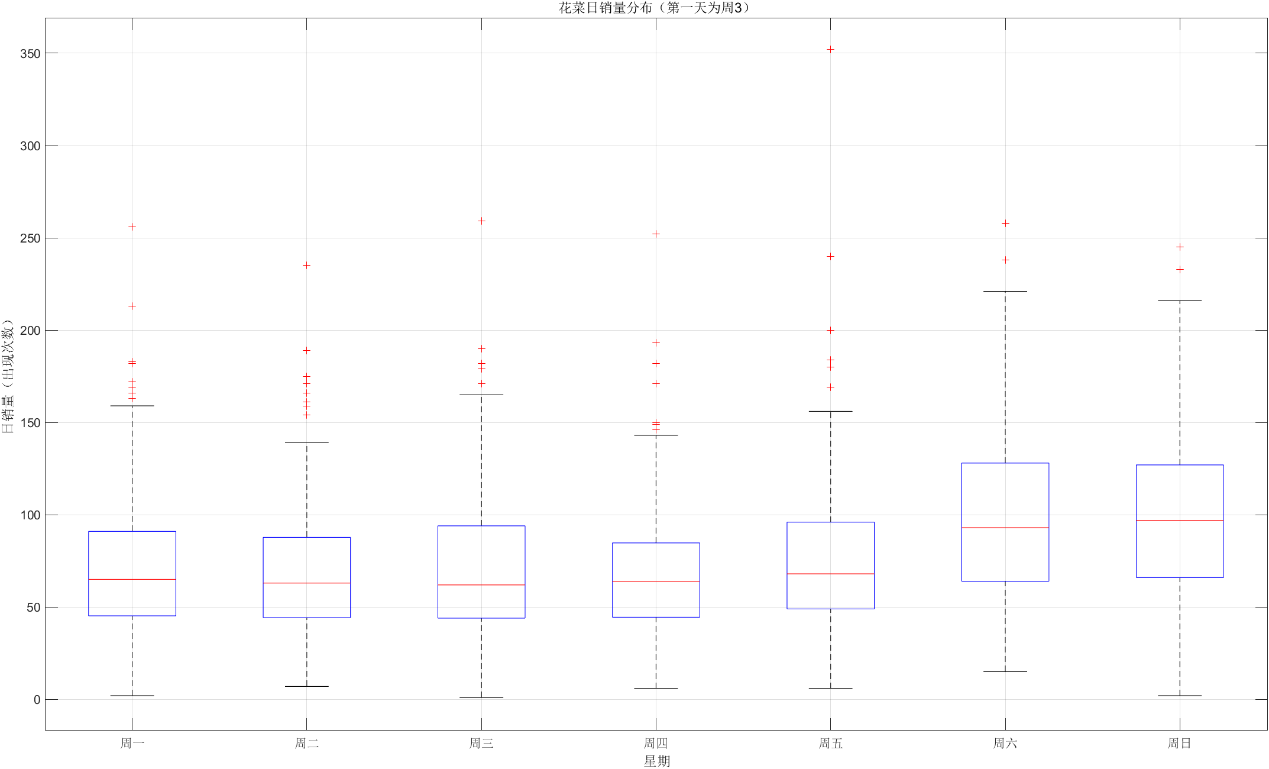
\includegraphics[width=0.8\textwidth]{花菜日销量分布(第一天为周3).png} 
    \caption{花菜类蔬菜日销量分布箱型图(第一天为周三)}
\end{figure}




\subsubsection{数据清洗整合}

首先,以“品类编码+销售日期”为入口,求出六类蔬菜的日均销量,并利用箱线图
对异常日销售量值剔除,保留观测范围内的数值。再求出所有观测值的平均值,
并且用该平均值代替异常值,中庸化处理以尽量减少未知因素对销量的异常影响。

对清洗后的销量进行汇总, 得到六大品类的日销量序列; 随后以7天为窗口滑动
求和, 生成周销量序列;以自然月为周期求和, 生成月销量序列。  

按小时、日、周、月四种粒度整理数据: 

(1)小时级: 提取原始流水中的“销售时间”字段, 汇总 0-23 点逐小时的日均销量图,  用于日内波动分析; 

(2)日级: 每日品类销量, 覆盖2020-07-01至2023-06-30共1095 d;   

(3)周级: 按ISO周历汇总, 共157周;   

(4)月级: 按自然月汇总, 共36个月. 

下面以花叶类蔬菜为例,展示其修复后的箱线图以及日均销量时间序列对比图。

\begin{figure}[H]
    \centering
    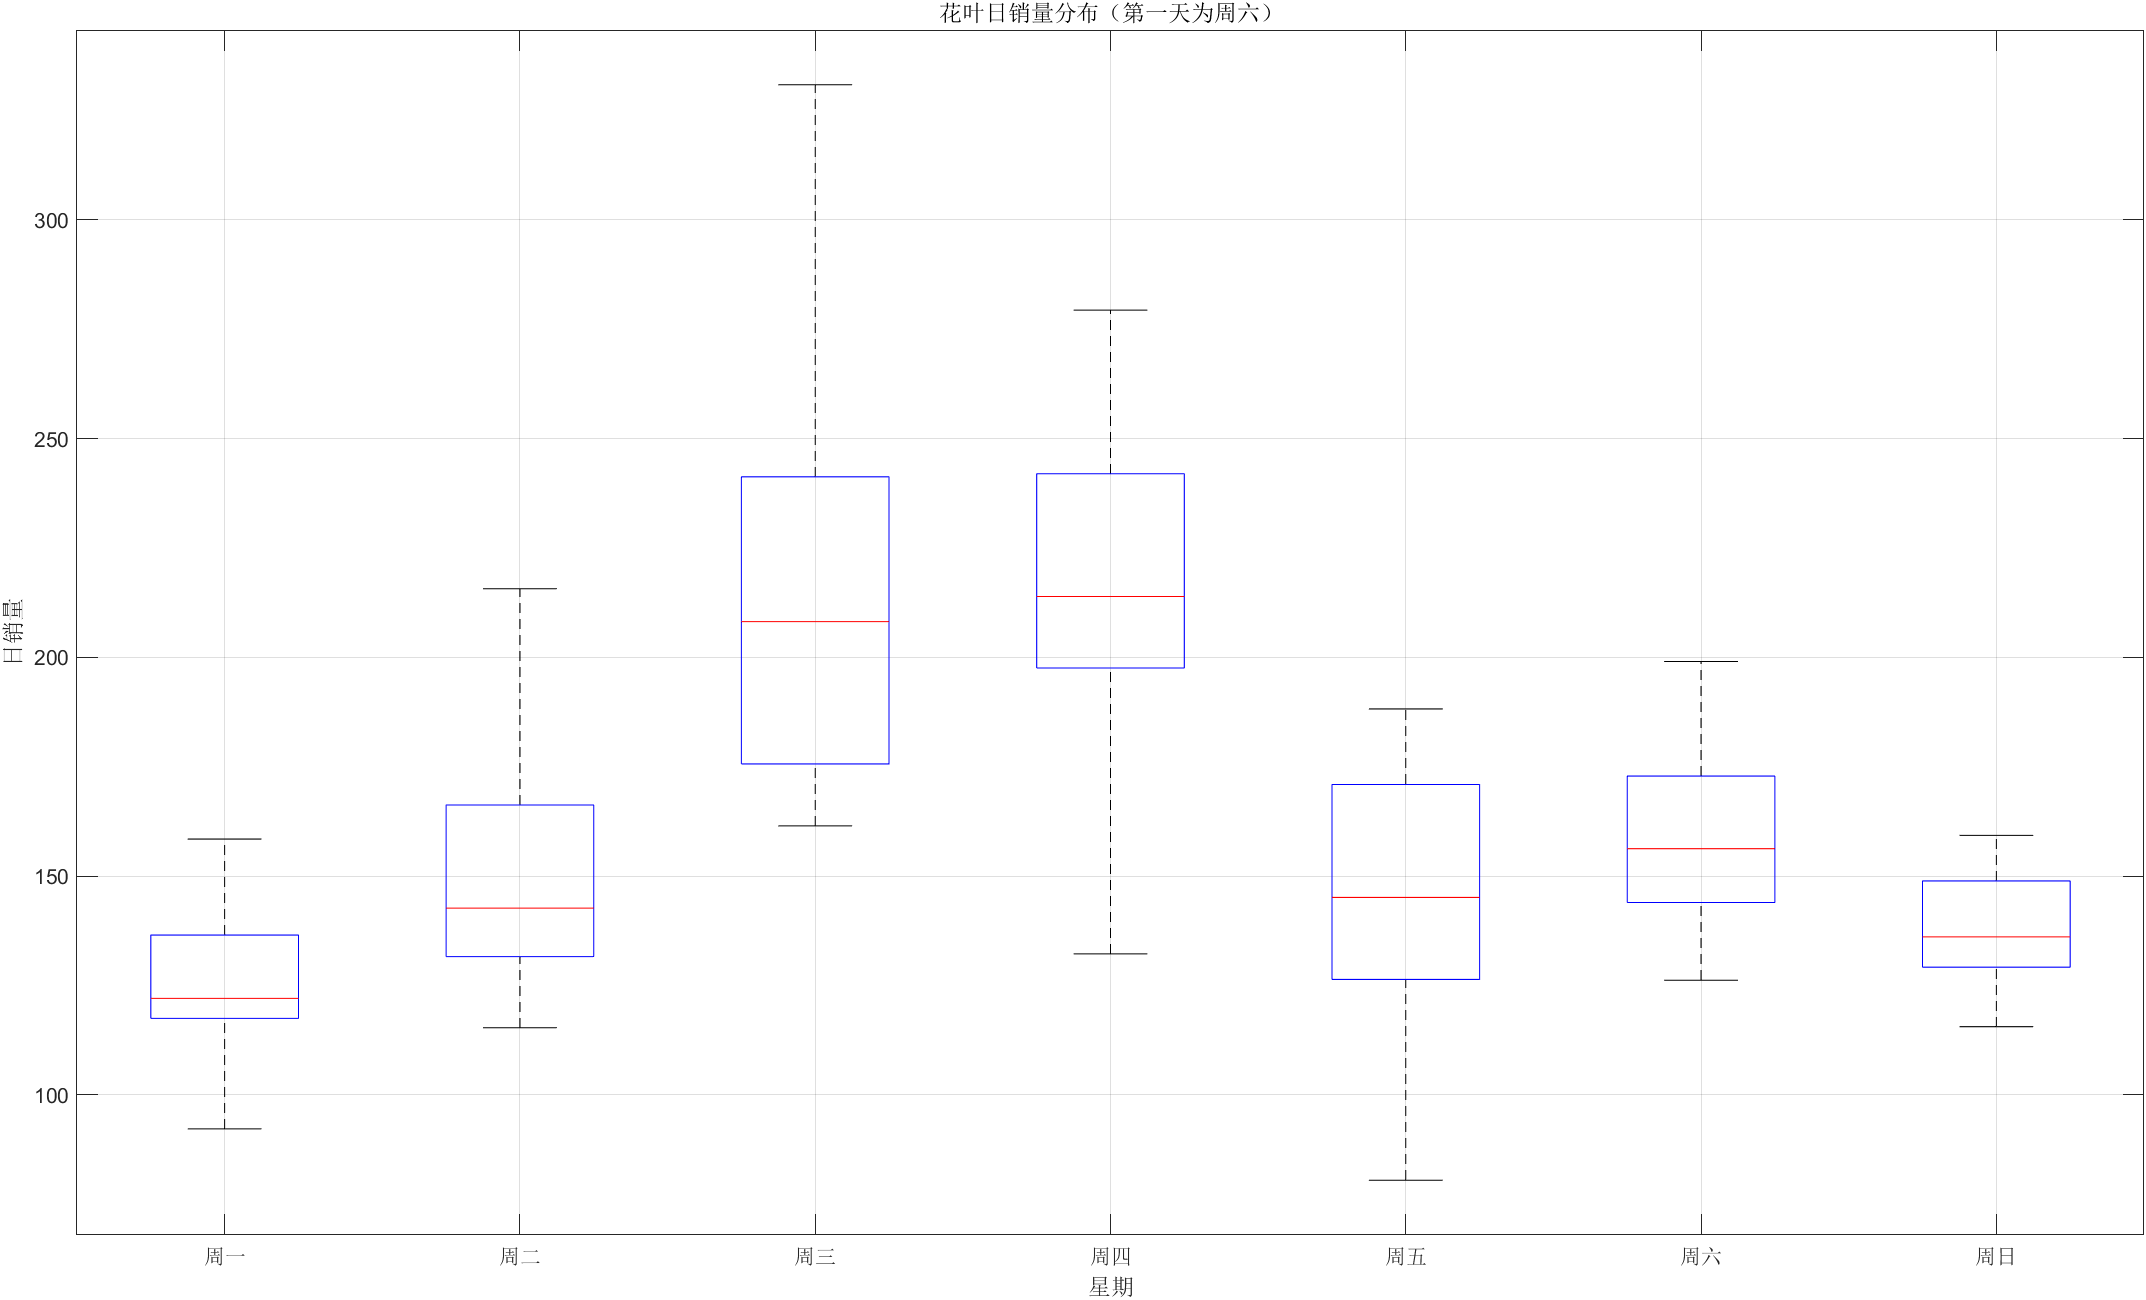
\includegraphics[width=0.6\textwidth]{修复后的花叶类蔬菜箱线图.png} 

    \caption{修复后的花叶类蔬菜箱线图}
    
    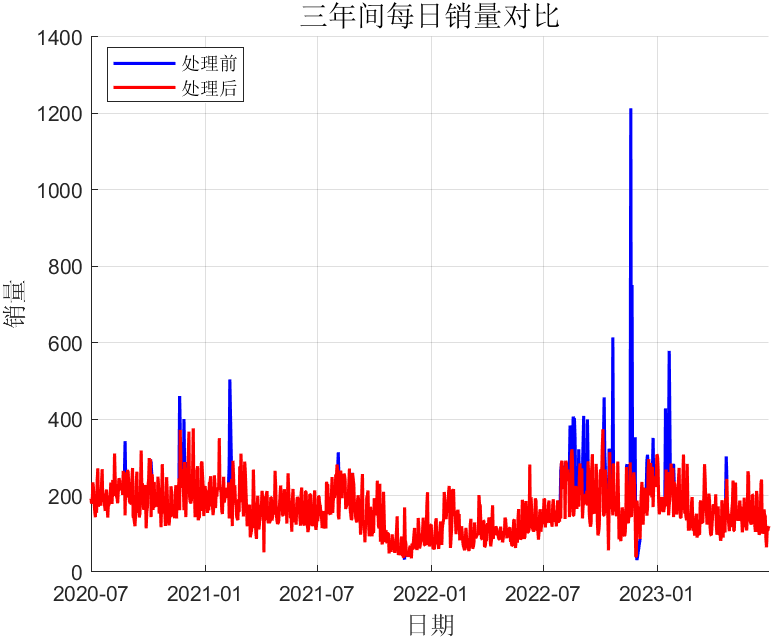
\includegraphics[width=0.6\textwidth]{日均销量时间序列对比图}

    \caption{修复后的花叶类蔬菜时间序列对比图}

\end{figure}

综合以上的内容,我们可以显著地看到修复后的三年间花叶类蔬菜的箱线图
异常值清零,所有数据已经修复到可观测范围内;日均销量时间序列图
更加平顺,极端值更少,这说明我们的预处理是有效的。并且清洗后的数据
不受极端值影响,为我们后续挖掘相互关系提供了一定帮助。

\subsection  {销售量的分布规律}

\subsubsection{多时间粒度的类间销售量比较}
\begin{figure}[H]
    \centering
    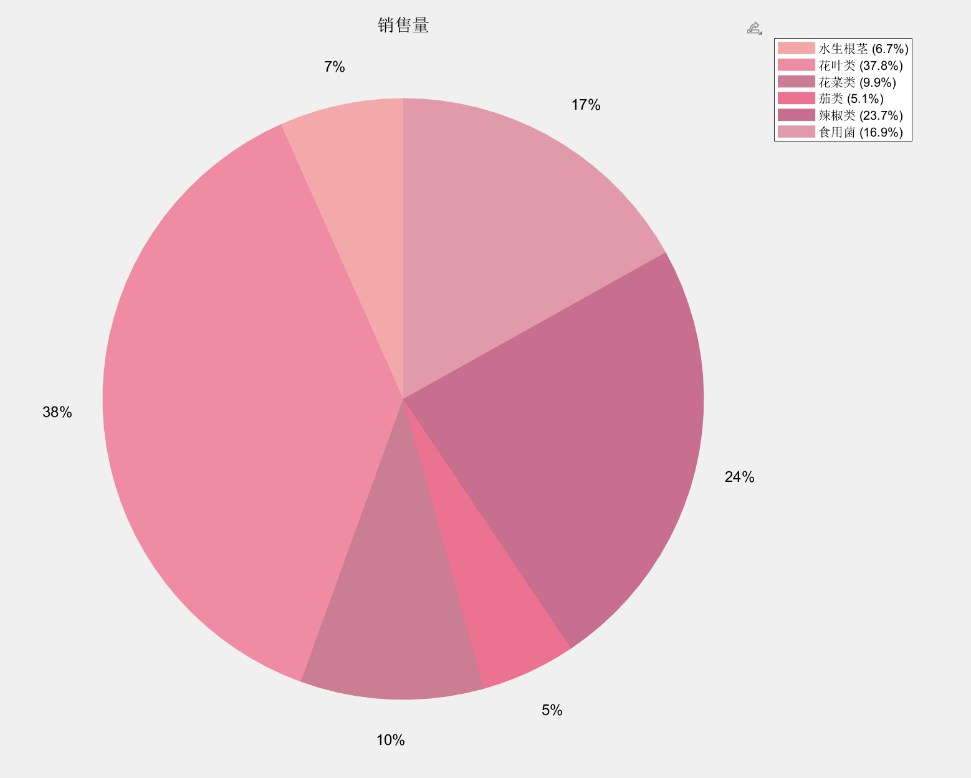
\includegraphics[width=0.6\textwidth]{销售量占比.png}
\end{figure}

在清洗后的数据基础上, 统计六大类别的蔬菜销售量占比. 花叶类总销量位于所有蔬菜品类销量之首, 
占比达到37.8\%;辣椒类和食用菌类的蔬菜占比分别达到23.7\%和16.9\%;花菜类、水生根茎类和茄类
总销量占比较少。
我们还需要得出具体的, 各品类的销售情况与相互关系. 由于附件所给数据为时间序列数据,因此
必须考虑时间效应,兼顾精细化需求,按月、日、小时不同的时间粒度,绘制时间序列图。


部分蔬菜三年逐月销量如下。观察发现,花菜类、花叶类、水生根茎类蔬菜在4、5月份销量较低,花菜在春秋季成熟较多,
辣椒多在6-8月成熟,水生根茎类多于秋季成熟。销售旺季与其现实生活成熟季节有较大关联性
,可见蔬菜销售对时间的依赖性。
\begin{figure}[H]
    \centering
    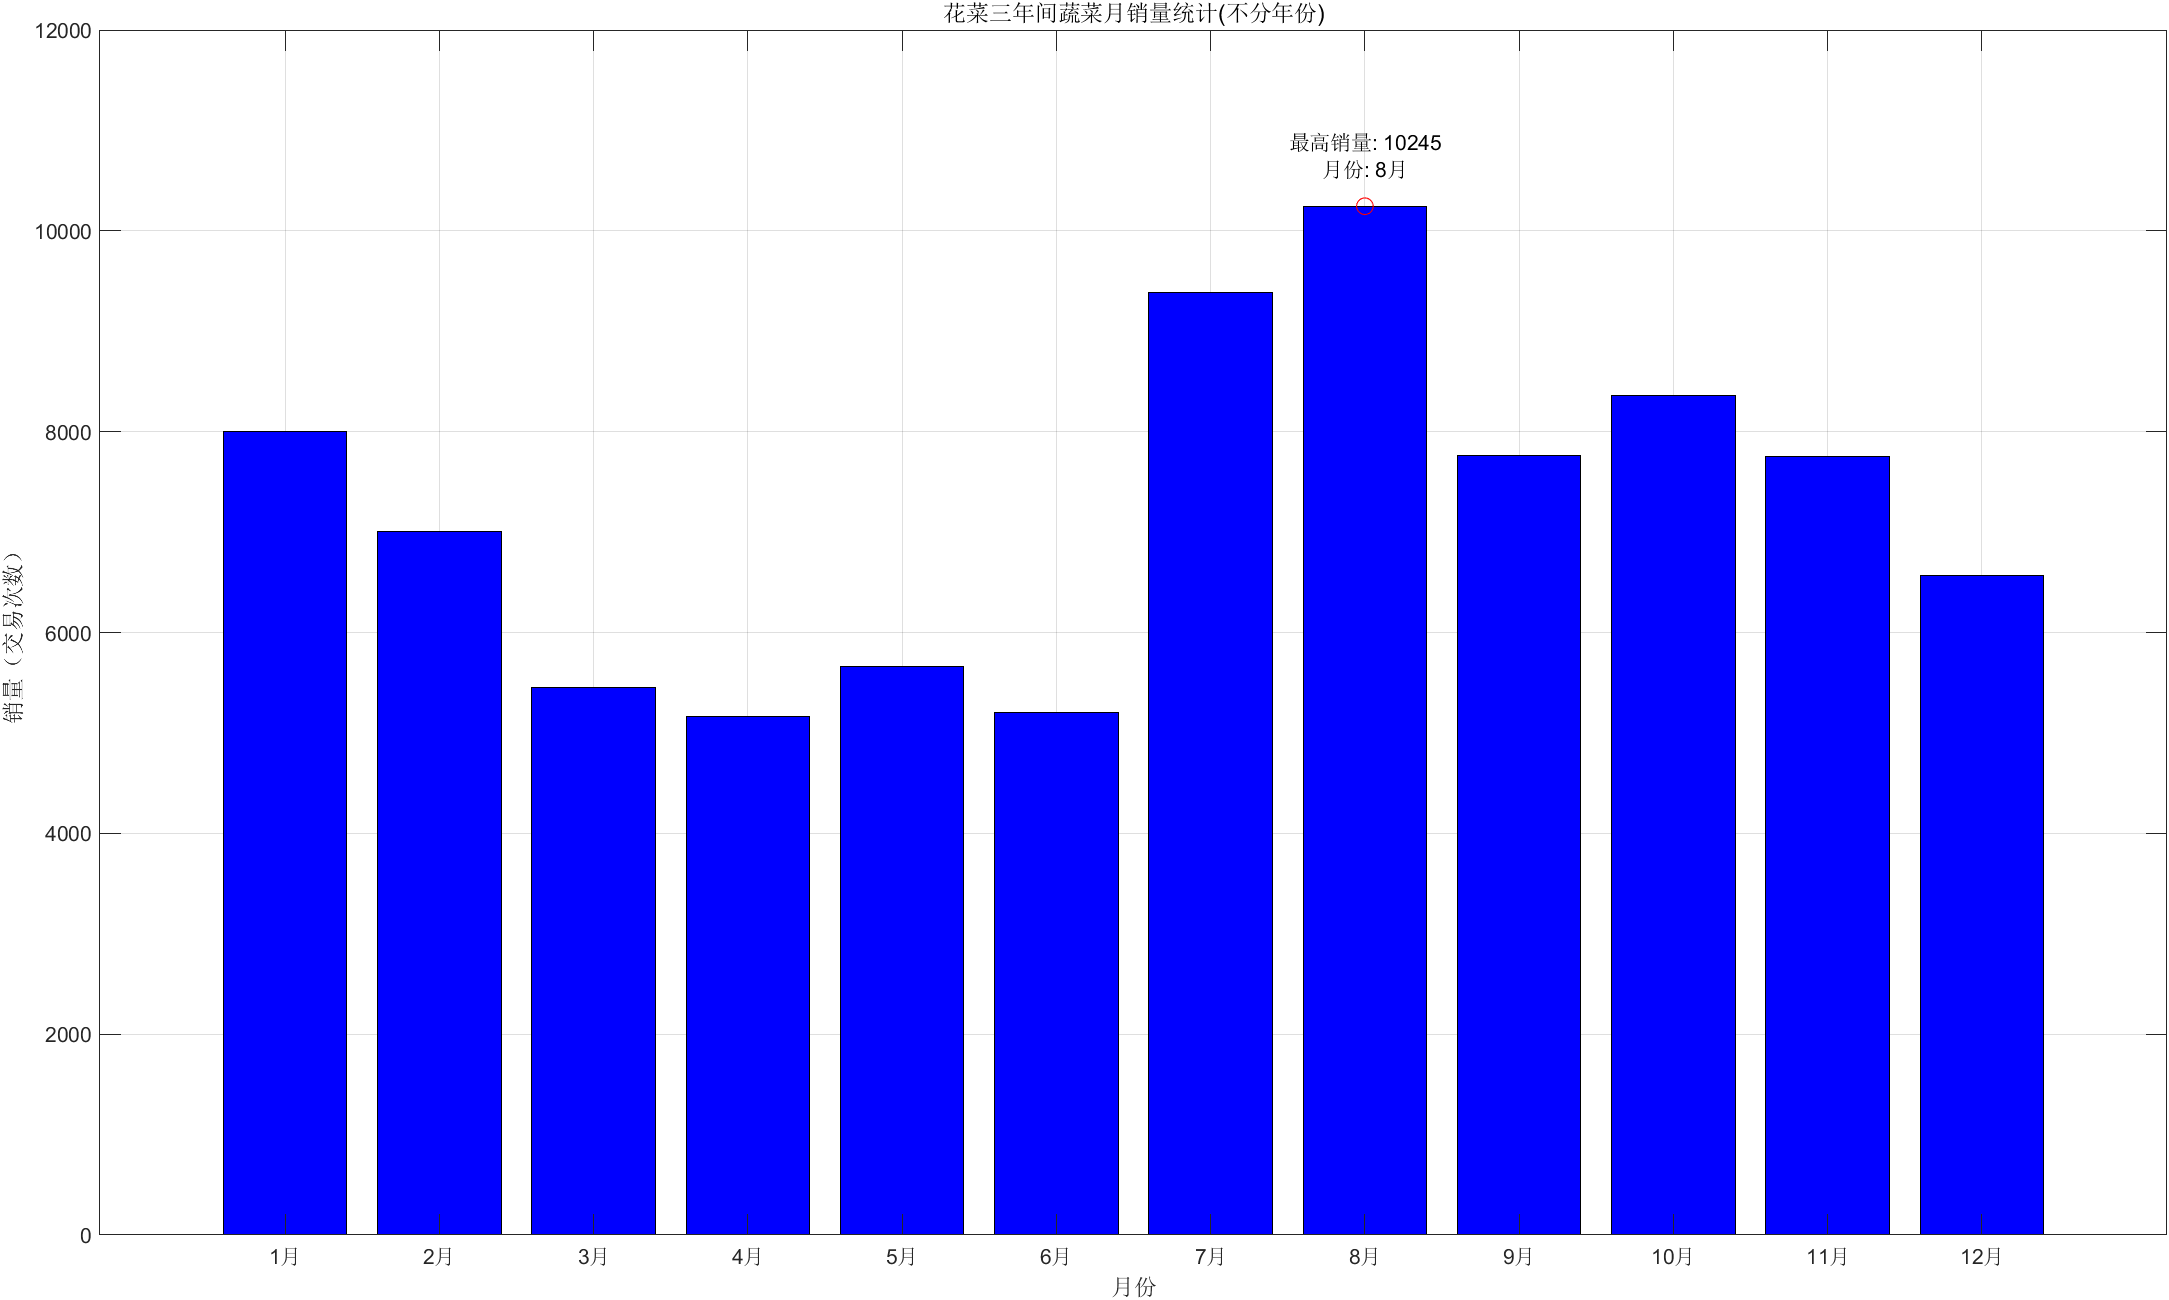
\includegraphics[width=0.6\textwidth]{三年花菜类月均销量.png} 
    \caption{三年花菜类月均销量}
\end{figure}

\begin{figure}[H]
    \centering
    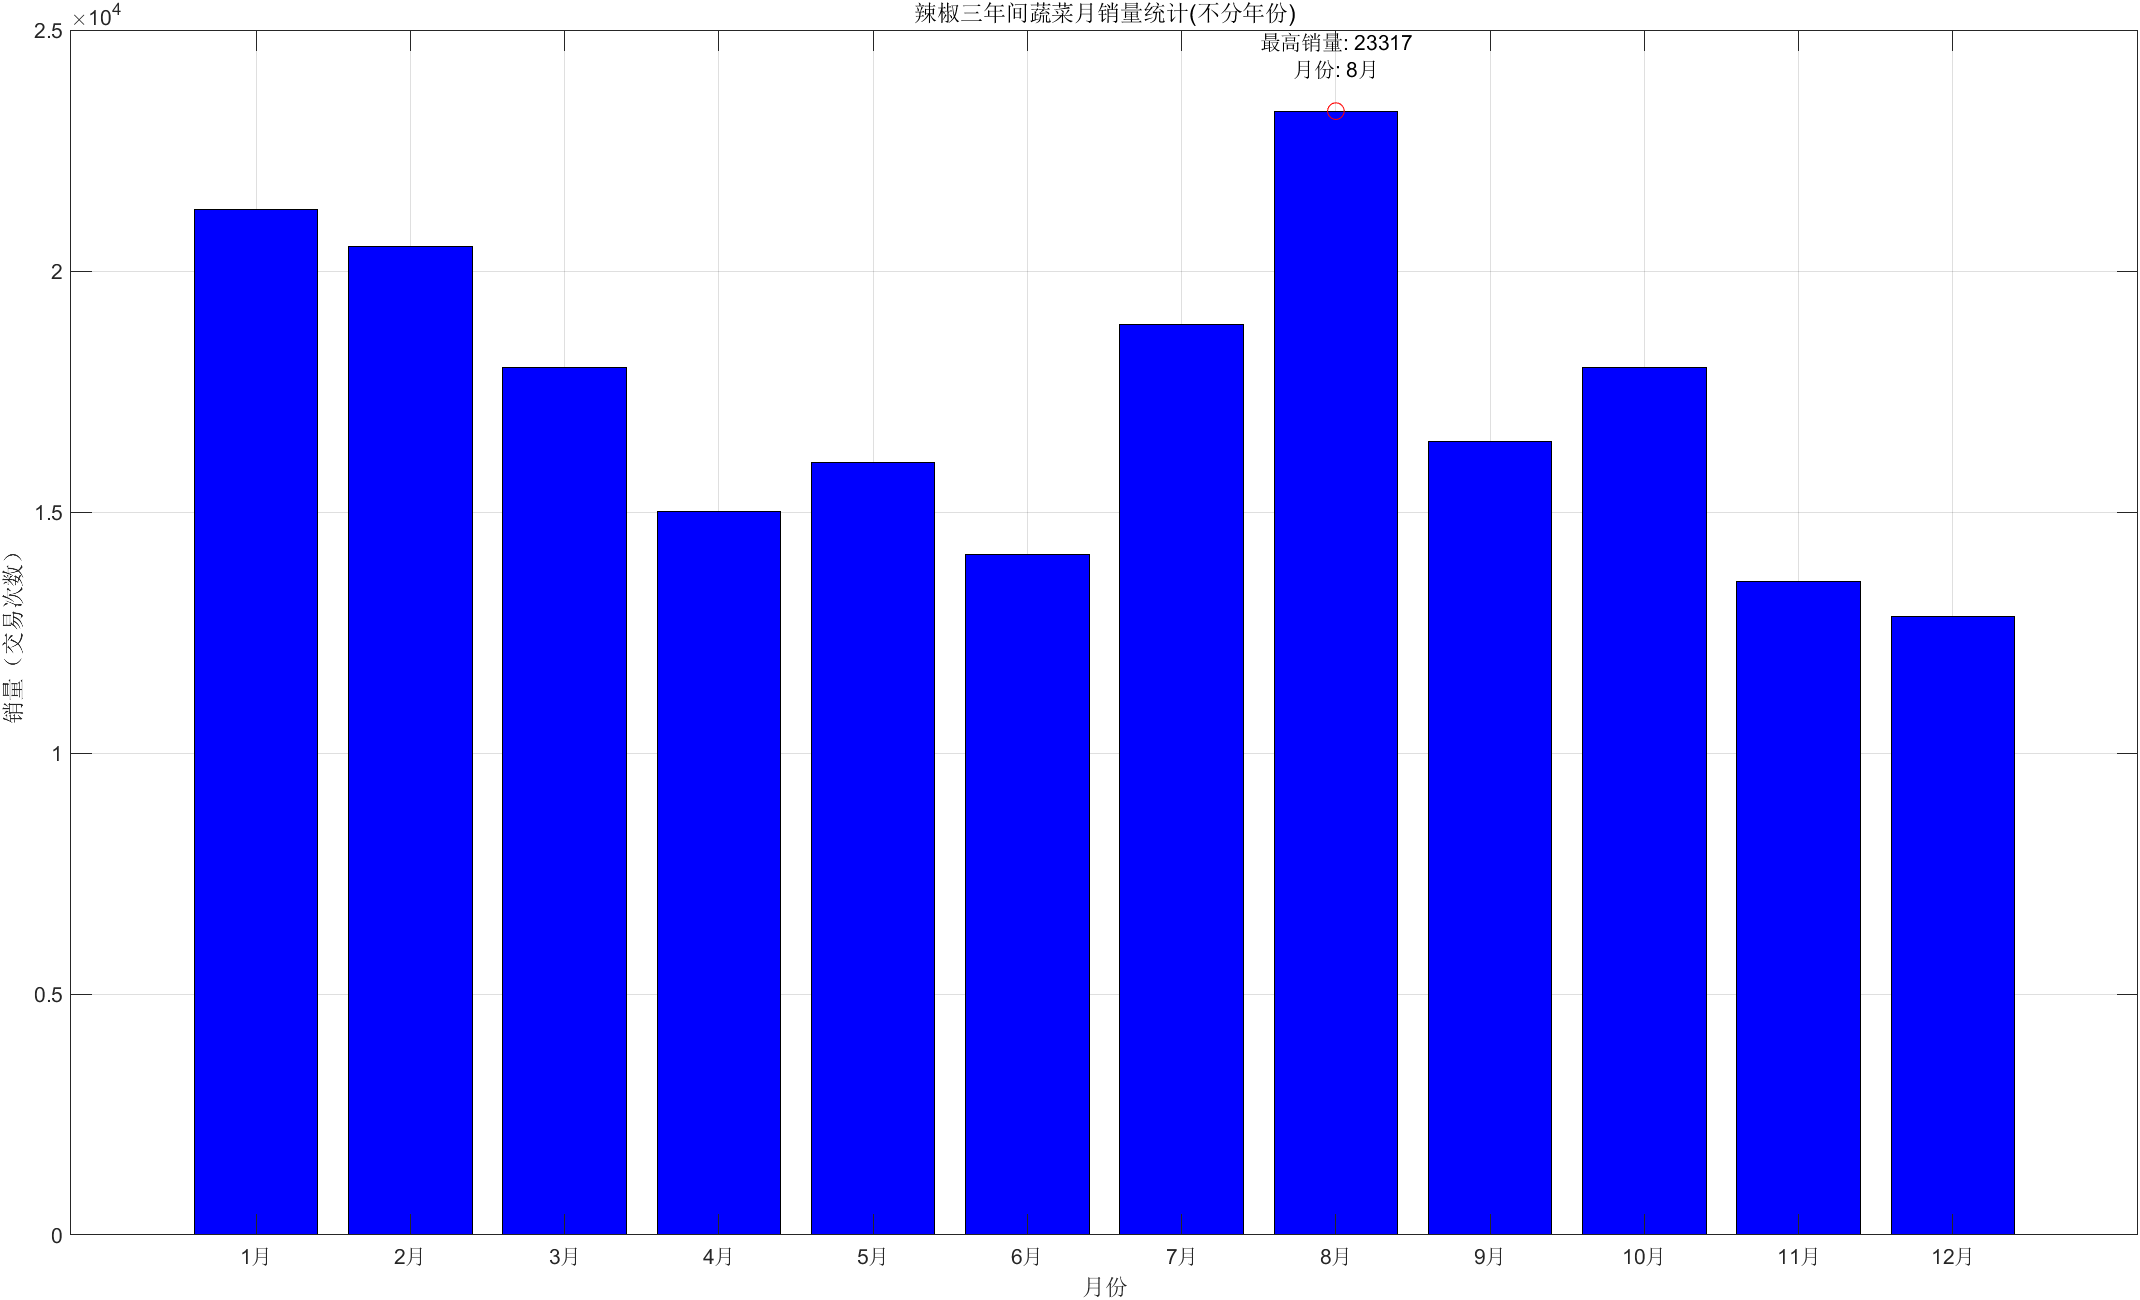
\includegraphics[width=0.6\textwidth]{三年辣椒类月均销量.png} 
    \caption{三年辣椒类月均销量}
\end{figure}

\begin{figure}[H]
    \centering
    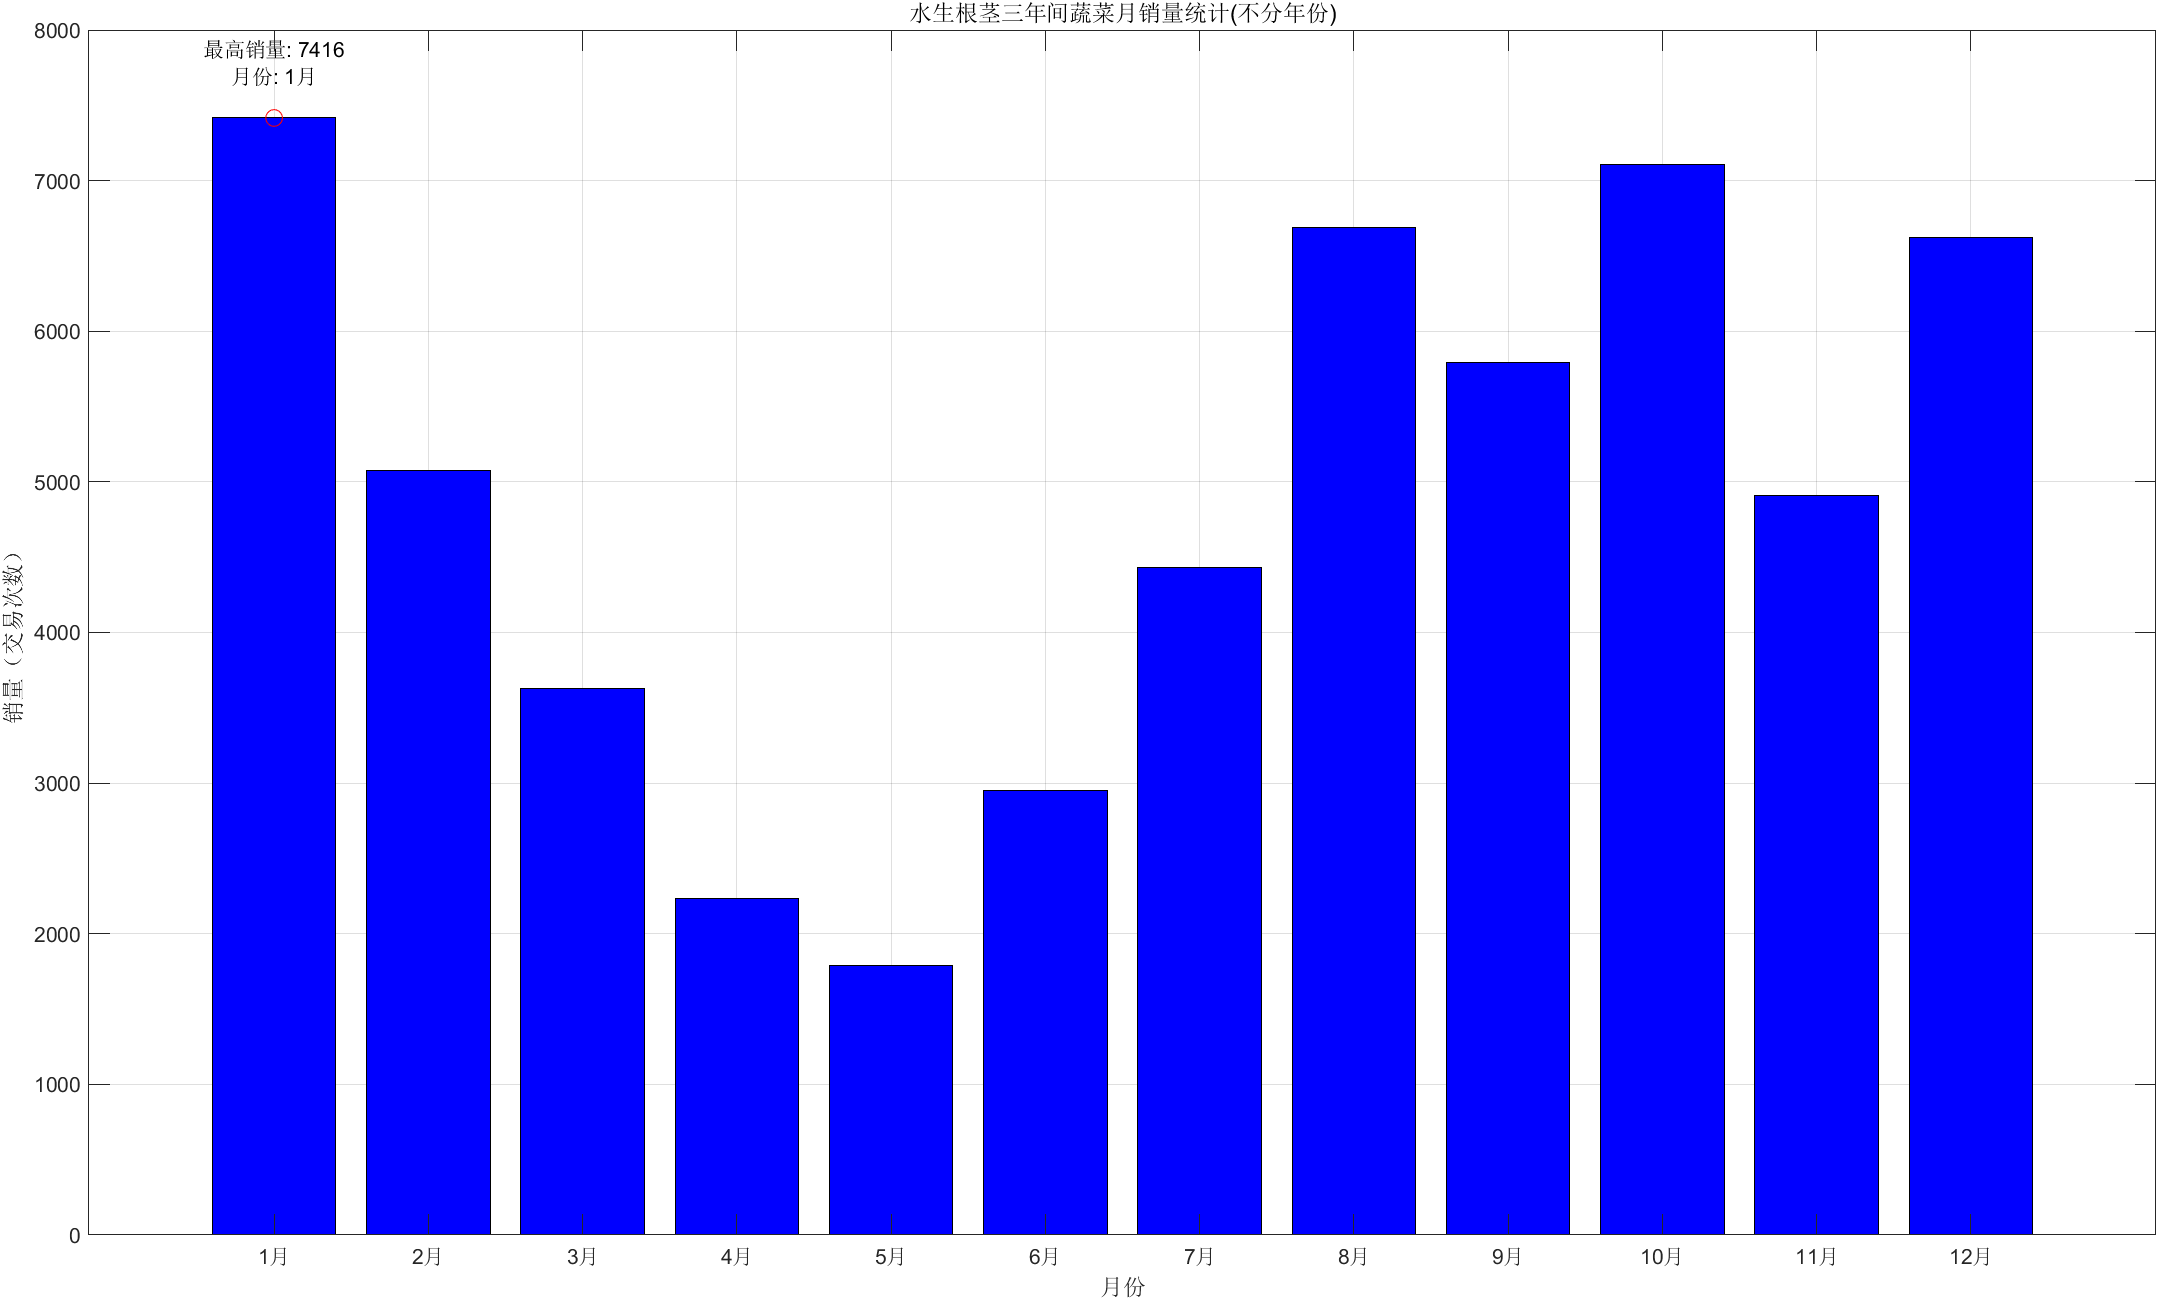
\includegraphics[width=0.6\textwidth]{三年水生根茎类月均销量.png} 
    \caption{三年水生根茎类月均销量}
\end{figure}



花叶蔬菜的三年总销量的日销量逐日分布折线比较图如下, 尽管2022年1月前后的日销量水平
与2021年、2023年同期水平相比较低, 该图仍然反映了一定的时间依赖性, 
如: 花叶类蔬菜日销售量1月左右销量步入低潮、6月后逐步销量步入升高。
这与花叶类蔬菜本身的季节性、周期性有关。此外,在销售中,总是出现“锯齿状”的
图样, 通过映射比较附件2中的日期数据, 发现节假日期间日销量会抬升, 周末总销量高于
工作日,反映出顾客集中采购行为增加;工作日销量平稳,各品类占比稳定。
总之,该图像反应花叶类销售呈现明显的时间依赖性,适合构建单变量时间序列。

\begin{figure}[H]
    \centering
    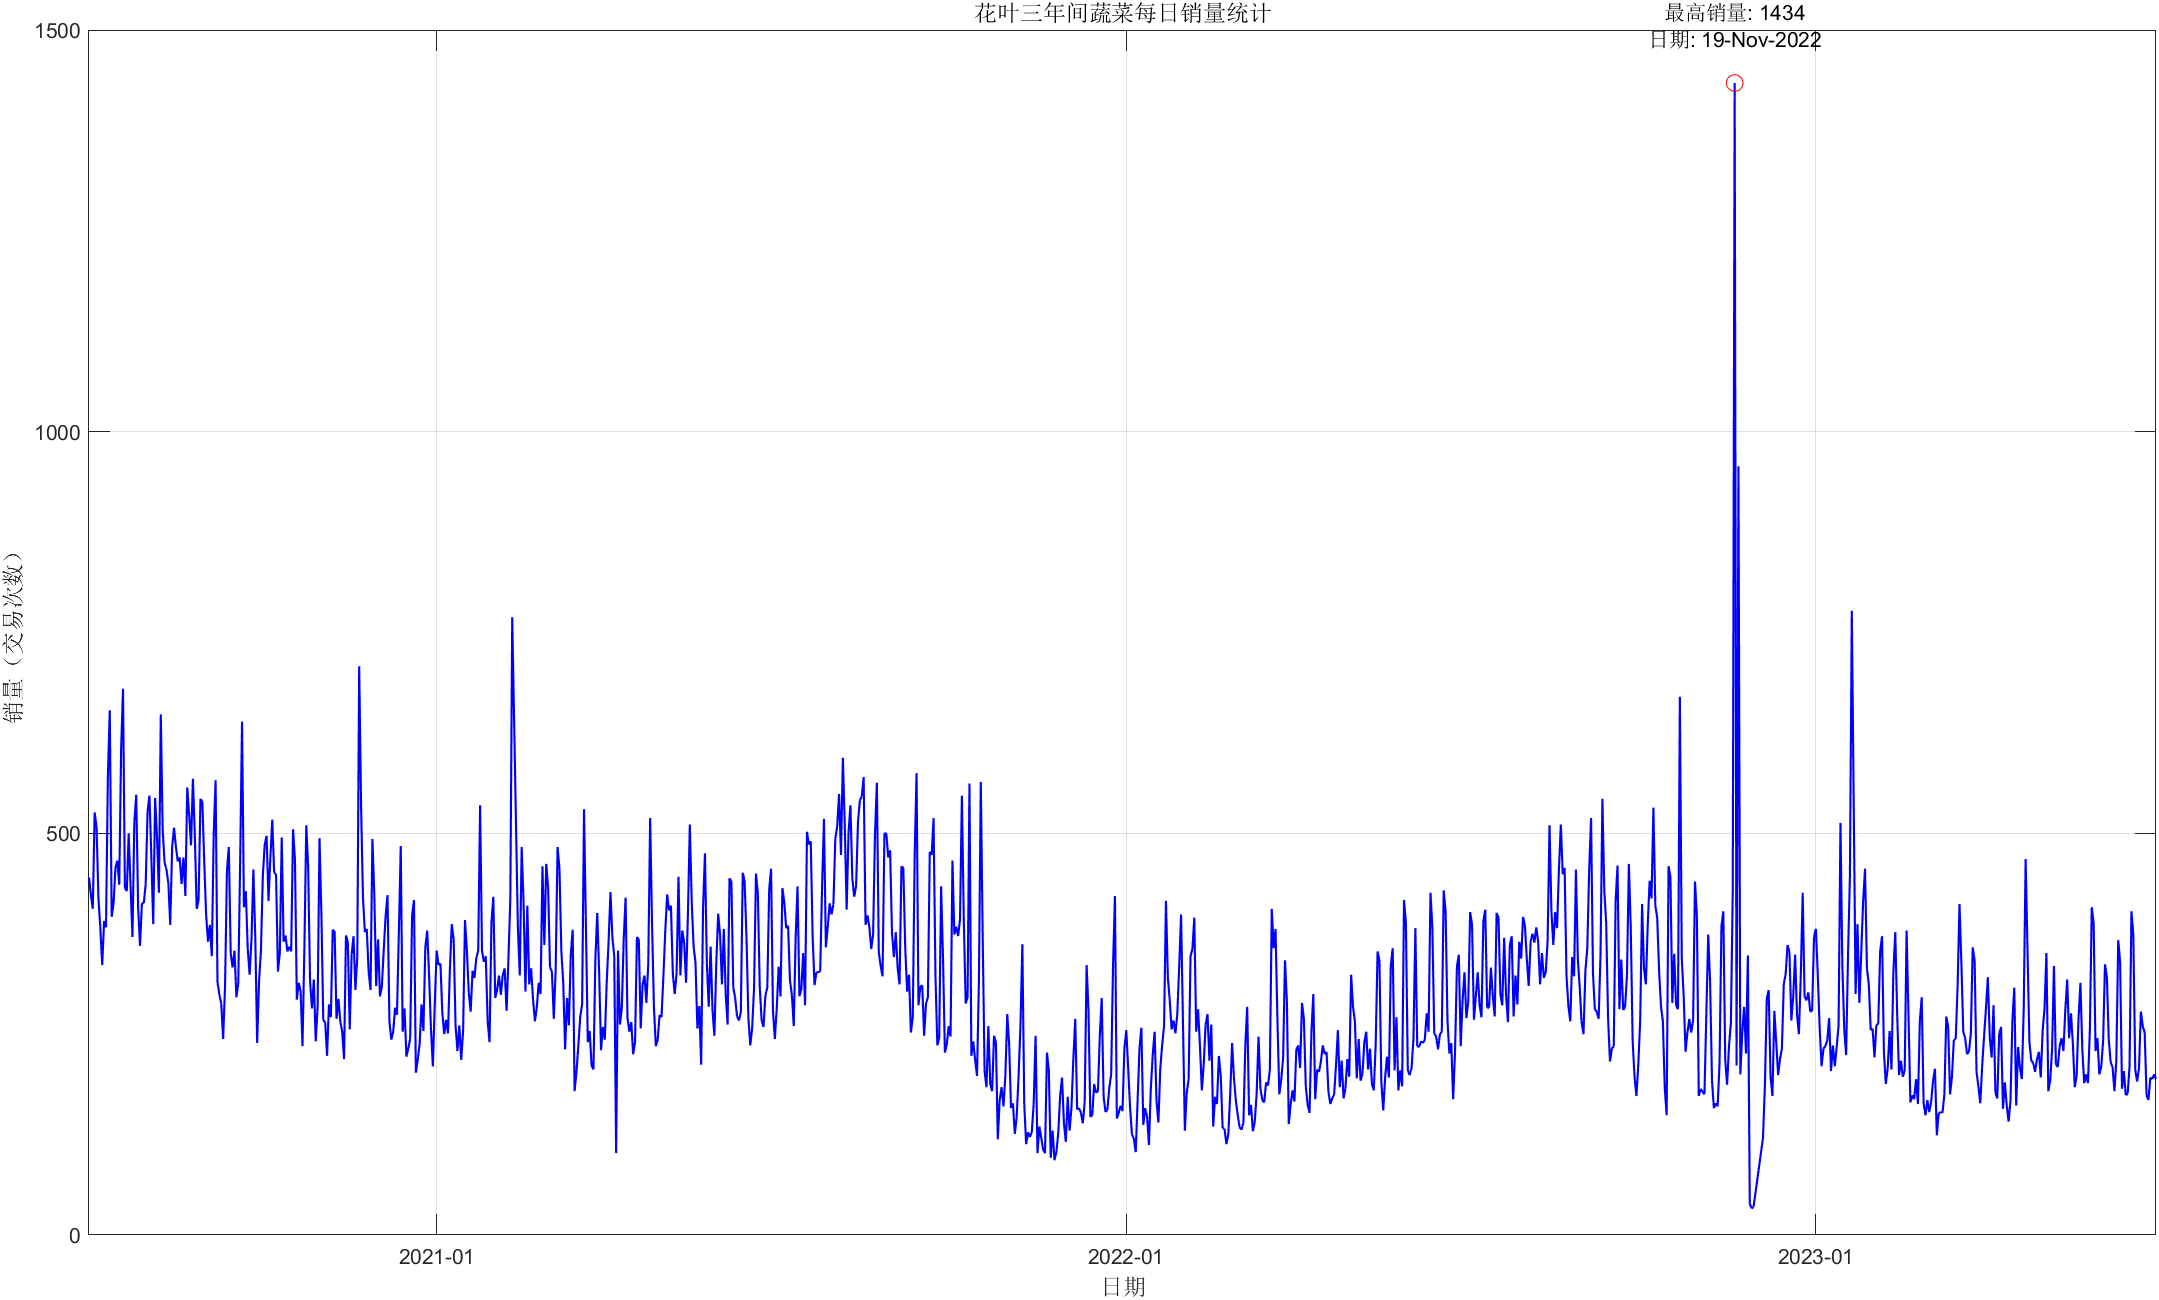
\includegraphics[width=0.8\textwidth]{花叶三年间蔬菜每日销量统计.png} 
    \caption{花叶类蔬菜三年每日销量统计折线图}
\end{figure}

\begin{figure}[H]
    \centering
    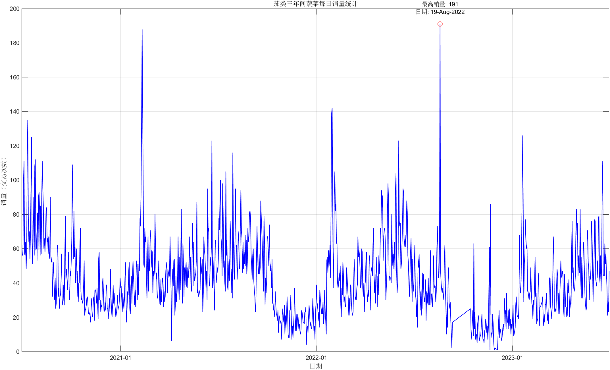
\includegraphics[width=0.8\textwidth]{其他品类日销量折线图1.png} 
    \caption{部分品类蔬菜三年每日销量统计折线图(一)}
\end{figure}

\begin{figure}[H]
    \centering
    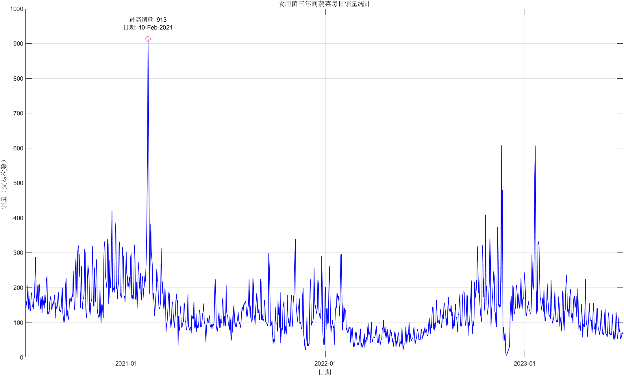
\includegraphics[width=0.8\textwidth]{其他品类日销量折线图2.png} 
    \caption{部分品类蔬菜三年每日销量统计折线图(二)}
\end{figure}

\begin{figure}[H]
    \centering
    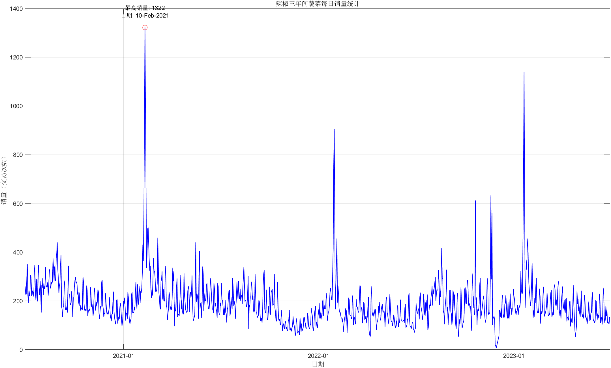
\includegraphics[width=0.8\textwidth]{其他品类日销量折线图3.png} 
    \caption{部分品类蔬菜三年每日销量统计折线图(三)}
\end{figure}

为了验证、推广上述分析, 其他类别蔬菜的缩略图如下. 茄类、水生根茎、辣椒类、食用菌类蔬菜的三年总销量的日销量逐日分布折线比较图如上. 从图中可以看出, 其峰值节点、日销售量趋势变化均呈现规律排布. 蔬菜品类的日销量具有显著的时间依赖性, 构成单变量时间序列, 并表现出明显的季节性、周期性和节假日效应. 而且, 长期来看各个品类销售占比较为稳定, 因此, 可针对各品类的日销量序列, 采用时间序列建模方法对其变动趋势进行模拟与预测.

\begin{figure}[H]
    \centering
    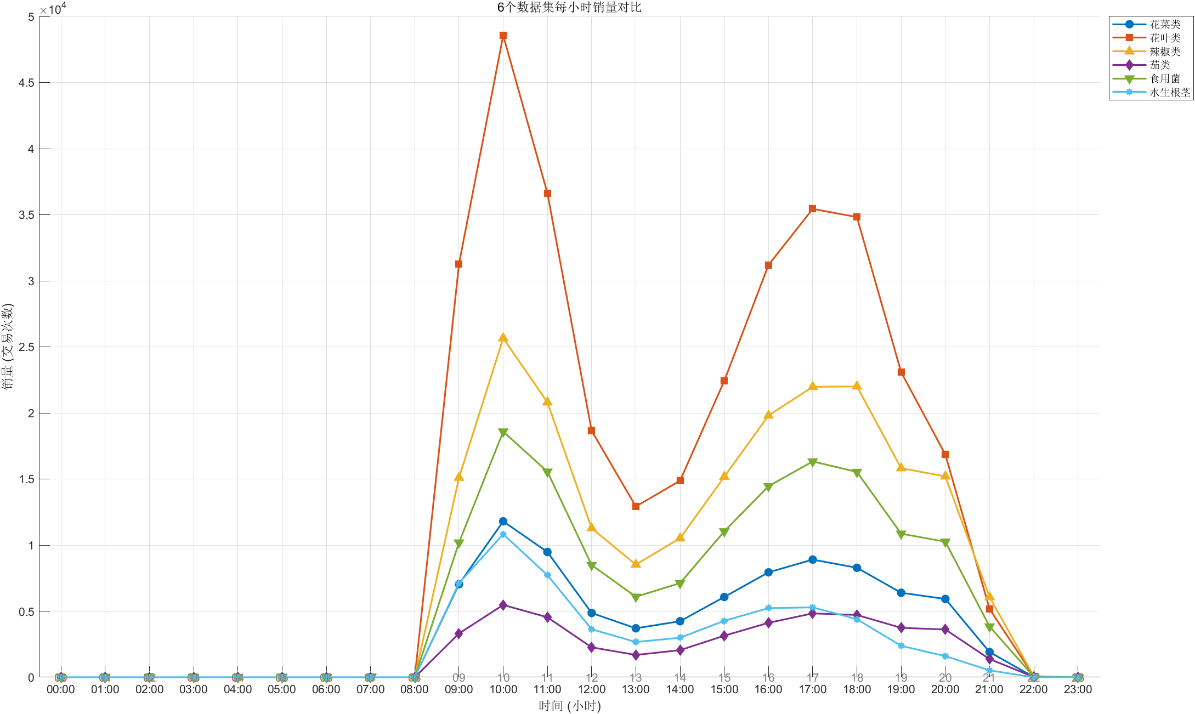
\includegraphics[width=0.8\textwidth]{6个数据集每小时销量对比.png} 
    \caption{六类蔬菜每小时销量对比图}
\end{figure}

六类蔬菜的三年总销量的平均日销量逐小时分布折线比较图如上. 花叶类蔬菜从早上8点至晚上10点持续有销量、且销售量折线基本覆盖其他类别蔬菜, 说明该类蔬菜是民众三餐常备菜品. 整体来看, 所有菜品的销量在上午10点和下午17点达到峰值, 恰好对应于午餐和晚餐前的备菜高峰, 符合现实情况.

\subsubsection{ARIMA 时间序列分析设计}

%\paragraph{时间序列建模}
ARIMA (自回归积分移动平均模型) 是时间序列分析中常用的预测模型, 适于处理非平稳时间序列数据. 
ARIMA模型由三部分组成, 记为ARIMA(p,d,q), 其中: 


(1) AR(p)自回归: 利用序列自身的滞后项(过去值)预测当前值, p为滞后项数。例如, p=2表示用前2期的值预测当前值. 

(2) I(d)积分: 通过对非平稳序列进行d次差分, 使其转化为平稳序列, d为差分次数 (通常d=0,1,2). 

(3) MA(q)移动平均: 关注自回归模型中误差项的累计, 利用序列的滞后误差项(预测误差)修正当前预测, q为误差项的滞后项数. 

根据需求分析维度, 以花叶类为例,建立以周为时间粒度的近三个月销量序列, 以捕捉周内需求波动、周度工作日—周末差异及季节性产地转换效应。  

建模流程如下:  

Step1 检查时间序列的连续性、绘制时序图  

Step2 平稳性检验, 若时序图显示非平稳 (有明显趋势), 需通过差分法通过ADF检验 (单位根检验)  

Step3 基于平稳后的序列, 绘制ACF (自相关函数)图和PACF (偏自相关函数)图定阶  

\begin{figure}[H]
    \centering
    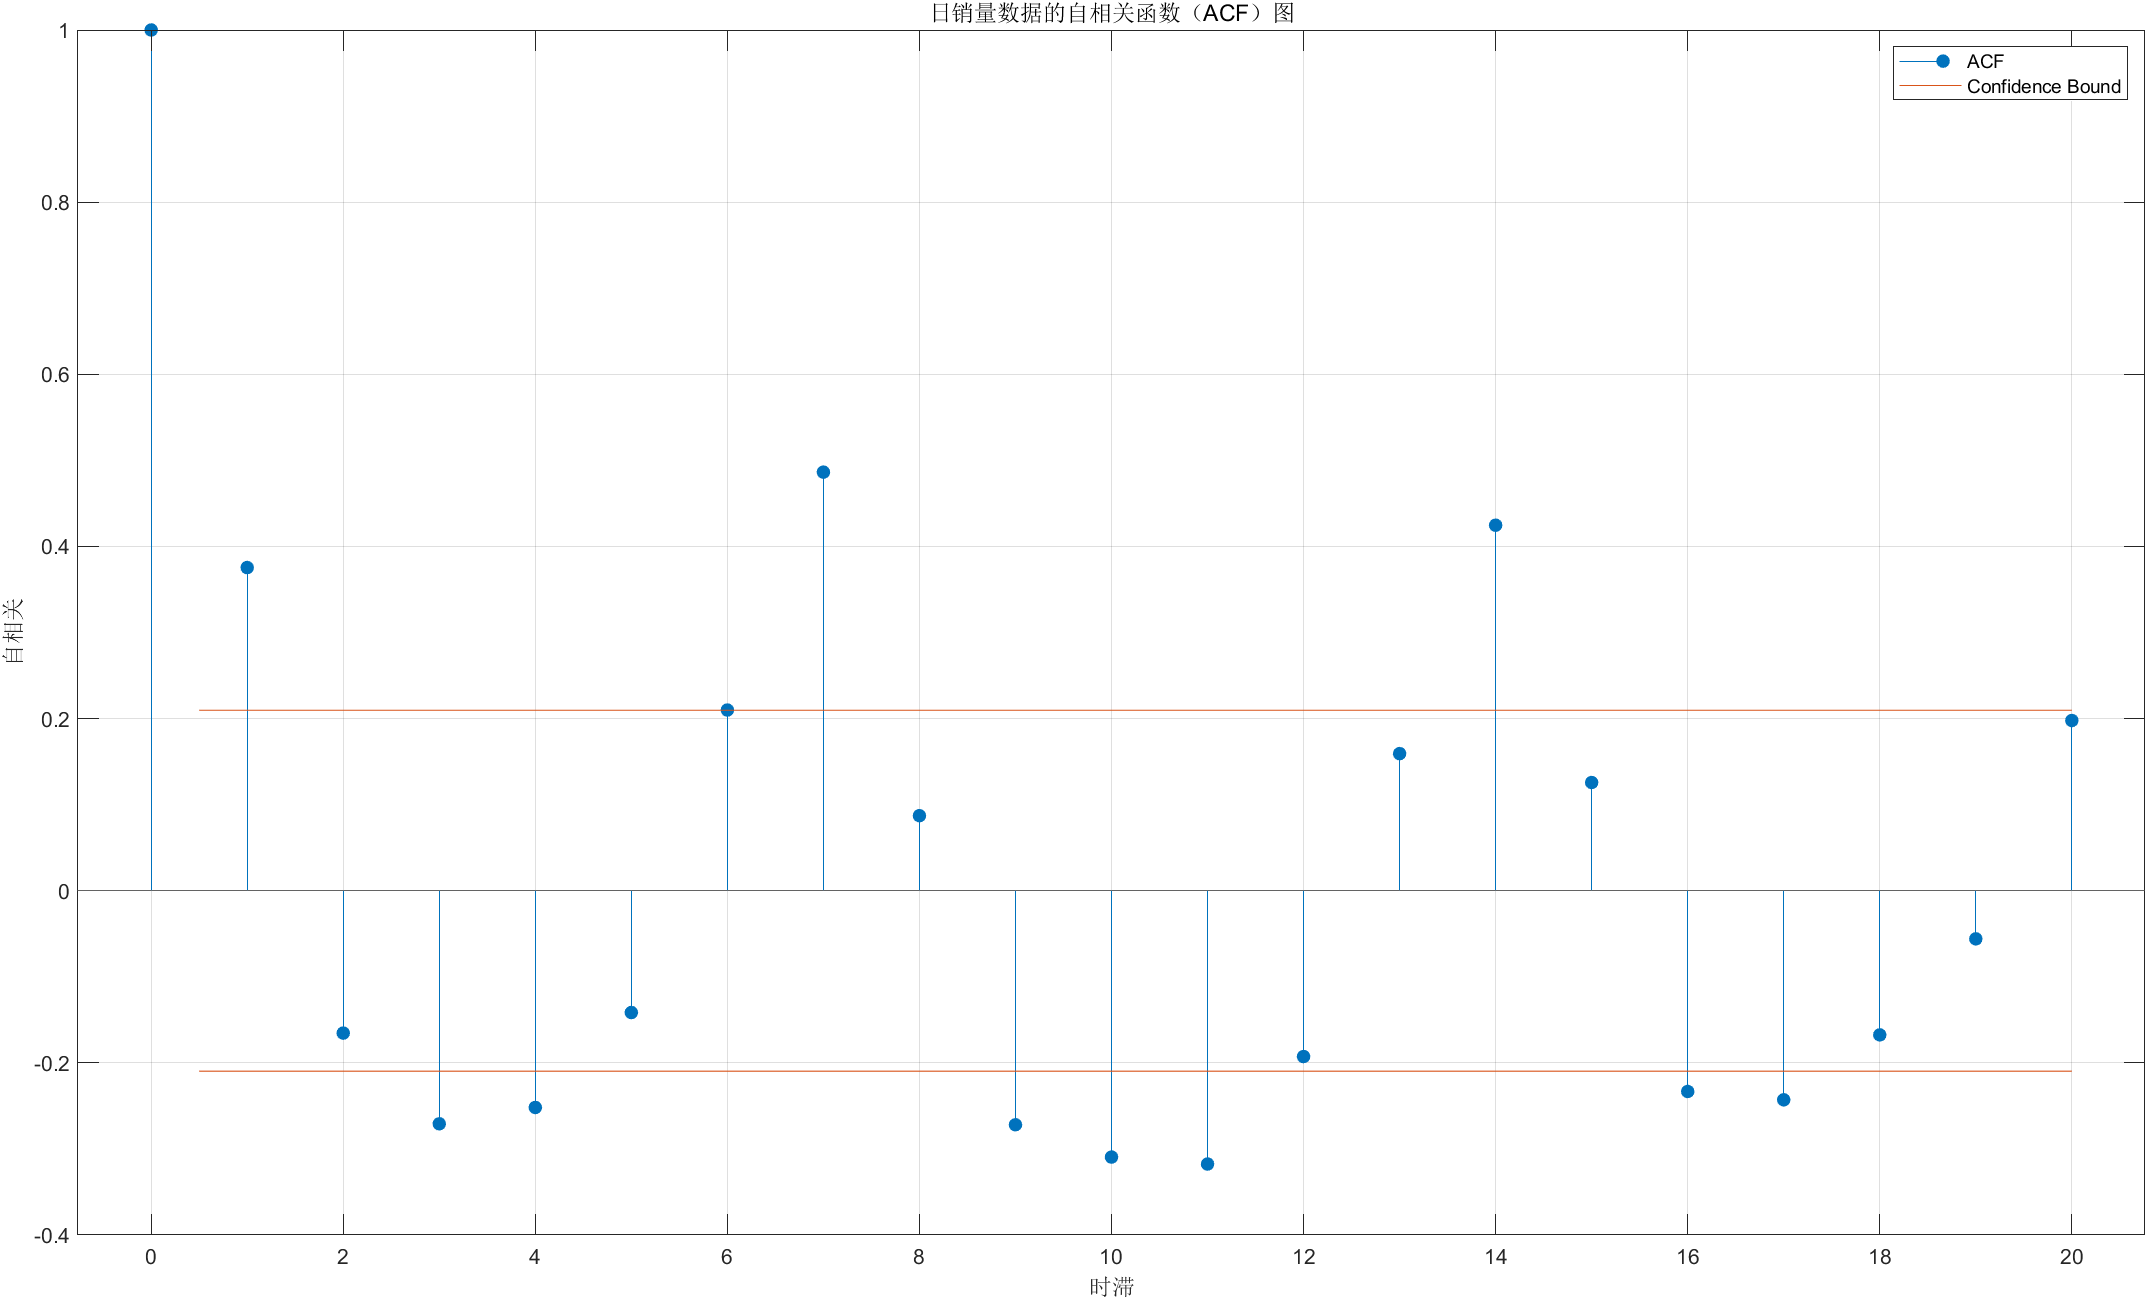
\includegraphics[width=0.8\textwidth]{花叶ACF图.png} 
    \caption{花叶类蔬菜销量ACF图}
\end{figure}

ACF 图用于衡量序列在不同滞后阶数下的线性相关性,反映序列当前值
与过去值(滞后 k 期)的整体关联程度,主要用于确定 MA (q) 的阶数。
在该图中,短期内滞后 1 期(即前 1 周)的自相关系数超出置信区间,
显著不为 0,说明近期销量对当前销量有直接影响
(如上周销量高,本周可能延续趋势)。由于数据以周为粒度且存在
周末 / 工作日差异,滞后 7 期、14 期等位置出现显著峰值,
反映周度周期性,表明民众的每周消费模式相似。


\begin{figure}[H]
    \centering
    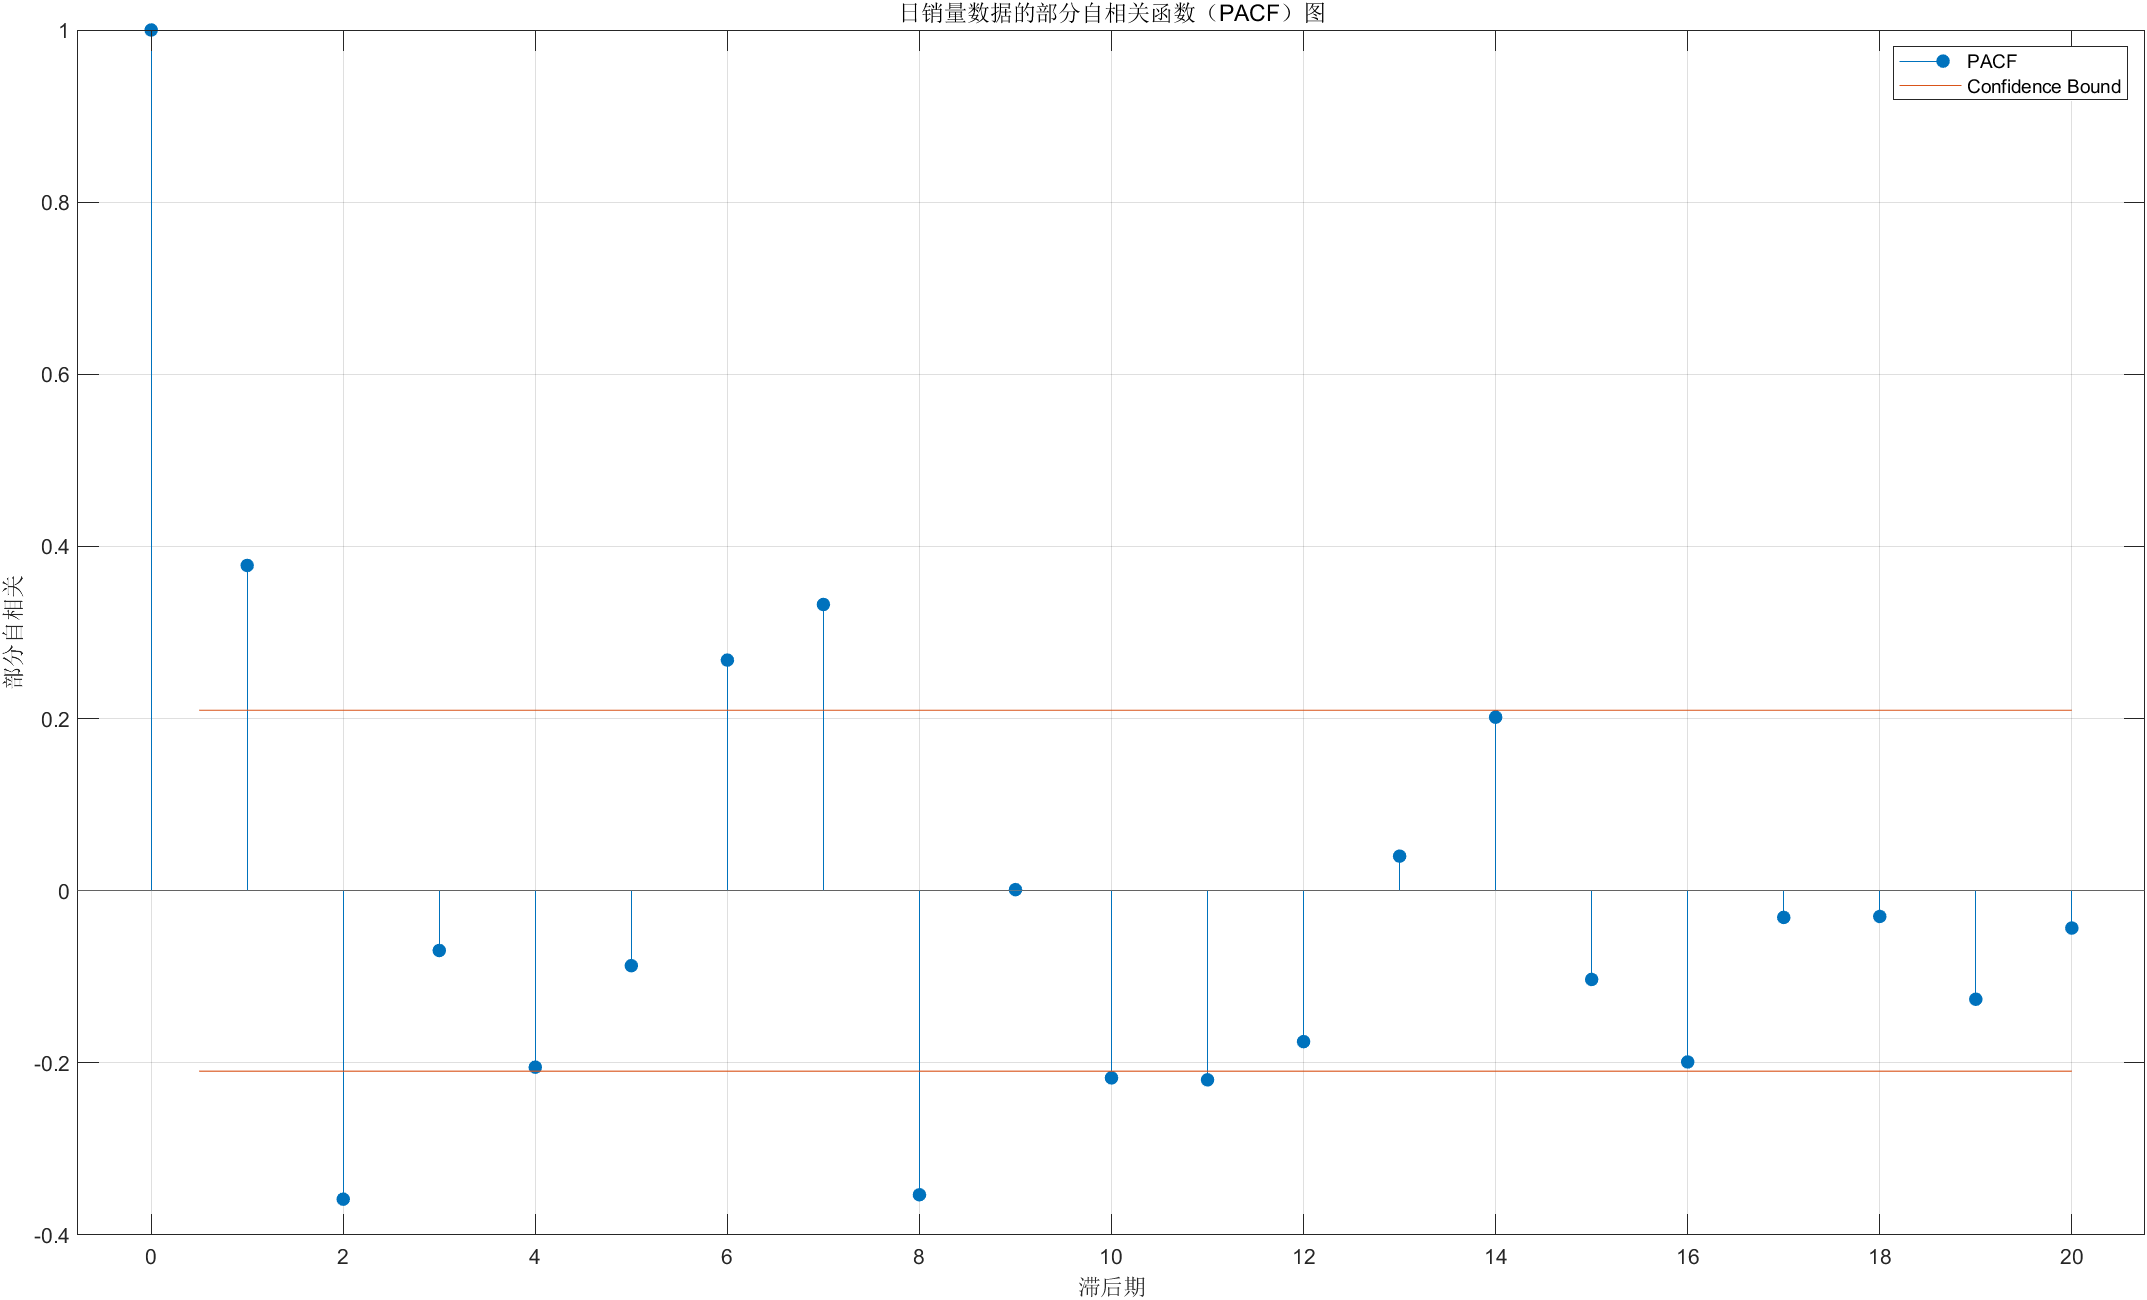
\includegraphics[width=0.8\textwidth]{花叶PACF图.png} 
    \caption{花叶类蔬菜销量PACF图}
\end{figure}

PACF 图用于衡量序列在控制中间滞后项影响后,
当前值与滞后 k 期值的净相关性,主要用于确定 AR (p) 的阶数。
在该图中,滞后 1-2 期的偏自相关系数显著不为 0,说明
在排除中间滞后项干扰后,前 1-2 周对当前销量
仍有直接影响,支持自回归项(AR)的存在。

综上所述,确定模型为 ARIMA (2,1,1)。


\subsection{销售量的相互关系}

\subsubsection{品类间的Pearson和Spearman相关系数分析}
为分析六大蔬菜品类 (花叶类、花菜类、水生根茎类、茄类、辣椒类、食用菌)间的
相互关系, 结合Pearson相关系数和Spearman等级相关系数, 从线性和单调两个维度
量化品类间的关联性, 以识别互补或替代关系。

\subsubsection{方法原理与适用性}
1. \textbf{Pearson相关系数}:   
核心原理基于协方差与标准差,衡量连续变量间的线性相关程度,公式为:  
\begin{equation}
r=\frac{Cov(X,Y)}{\sigma_x \cdot \sigma_y}
\end{equation}  

其中$Cov(X,Y)$为协方差,$\sigma_x$和$\sigma_y$分别为变量$X$和$Y$的标准差.  
该方法适用于变量为连续型, 数据近似服从正态分布或
样本量$n>30$, 且关系呈线性 (点图呈直线趋势)的情况。

%局限性: 对异常值敏感, 需通过数据预处理剔除极端值. 

2. \textbf{Spearman等级相关系数}:   
核心原理基于秩次转换, 将数据按大小排序为等级, 衡量单调关系 (同增或同减趋势), 公式为: 
\begin{equation}
\rho=1-\frac{6\sum d_i^2}{n(n^2-1)}
\end{equation}  
其中$d_i$为两变量秩次差,$n$为样本量。该方法适用于变量为连续型或有序分类
 (如销量等级), 关系单调但非线性, 数据非正态或含异常值时更稳健。

\subsubsection{分析流程设计}
%\begin{enumerate}
    Step1 数据预处理: 聚合品类日销量数据, 缺失值以0填充 (无销售日), 
    异常值通过四分位距 (IQR)法处理 (替换为均值); 标准化销量以消除量纲影响。
    该步骤在4.1部分已经进行。
   
    Step2 相关系数计算与检验: 分别计算日销量的Pearson $r$与
    Spearman $\rho$。反映短期波动关系。 
    
    Step3 显著性检验: 通过$t$-检验 
    ($t=\frac{r(n-2)}{\sqrt{1-r^2}}$,自由度$df=n-2$)验证相关性,
    $P<0.05$视为显著相关 (非随机误差)。
    
    Step4 通过下列准则确定关系: 
   
    (1)替代关系:显著负相关 ($r<0$或$\rho<0$, $p<0.05$), 如辣椒类与花叶类竞争消费者预算; 

    (2)互补关系:显著正相关 ($r>0$或$\rho>0$, $p<0.05$), 如花菜类与食用菌常搭配销售;  

    (3)无关性:$|r|$或$|\rho|$接近0或$p≥0.05$.

%\end{enumerate}

\subsubsection{相关系数矩阵} 
\paragraph{Pearson相关系数矩阵}
\begin{table}[H]
\centering
\begin{tabular}{c c c c c c c}
\toprule
品类 & 水生根茎 & 花叶类 & 花菜类 & 茄类 & 辣椒类 & 食用菌 \\
\midrule
水生根茎 & 1 & 0.42 & 0.38 & -0.15 & 0.38 & 0.62 \\
花叶类 & 0.42 & 1 & 0.60 & 0.37 & 0.66 & 0.61 \\
花菜类 & 0.38 & 0.60 & 1 & 0.22 & 0.48 & 0.49 \\
茄类 & -0.15 & 0.37 & 0.22 & 1 & 0.22 & -0.01 \\
辣椒类 & 0.38 & 0.66 & 0.48 & 0.22 & 1 & 0.57 \\
食用菌 & 0.62 & 0.61 & 0.49 & -0.01 & 0.57 & 1 \\
\bottomrule
\end{tabular}
\end{table}

\paragraph{Spearman相关系数矩阵}
\begin{table}[H]
\centering
\begin{tabular}{c c c c c c c}
\toprule
品类 & 水生根茎 & 花叶类 & 花菜类 & 茄类 & 辣椒类 & 食用菌 \\
\midrule
水生根茎 & 1 & 0.42 & 0.39 & -0.19 & 0.33 & 0.61 \\
花叶类 & 0.42 & 1 & 0.63 & 0.32 & 0.59 & 0.60 \\
花菜类 & 0.39 & 0.63 & 1 & 0.24 & 0.43 & 0.46 \\
茄类 & -0.19 & 0.32 & 0.24 & 1 & 0.16 & -0.09 \\
辣椒类 & 0.33 & 0.59 & 0.43 & 0.16 & 1 & 0.53 \\
食用菌 & 0.61 & 0.60 & 0.46 & -0.09 & 0.53 & 1 \\
\bottomrule
\end{tabular}
\end{table}

通过上述两表分析,可得出下列结论:
1.花叶类蔬菜与其他类别蔬菜的相关系数整体较大,
表明花叶类与它们的正相关性较强。购买其他蔬菜时,
很有可能会购买花叶类蔬菜。

2.“食用菌、辣椒类和花叶类蔬菜”之间的相关系数的绝对值较大,推测民众购买
花叶类蔬菜时,最有可能连带购买的是辣椒类和食用菌。商超可据此互补性搭配销售。

换而言之,民众会选择固定的蔬菜搭配,如辣椒搭配花叶类蔬菜,
两个系数矩阵表明部分蔬菜品类间具有较强的相关性;
除此之外,相关系数低于0.4,可认为是二者之间的相关性并不明显。

3.表中存在部分相关系数为负的情况,如食用菌和茄类,可认为二者销售
时相关性近似于0,呈现为无关性。

\subsection{单品聚类分析:群体特征与关系分组}
\subsubsection{方法原理与优势}

\textbf{核心原理}: 采用K-means聚类算法, 通过最小化簇内平方误差 (SSE) 划分单品, 公式为: 
\begin{equation}
SSE=\sum_{i=1}^{K}\sum_{x\in C_i}||x-\mu_i||^2
\end{equation}  
其中$\mu_i$为第$i$个簇的质心,$x$为数据点,欧氏距离度量相似性:  
\begin{equation}
d(x,y)=\sqrt{\sum (x_i-y_i)^2}
\end{equation}

 该方法可处理单品销量、价格、季节性指标等高维数据, 
 通过分组降低复杂度, 识别隐性关联 (如“时令蔬菜群”),
 弥补相关系数仅限两两关系的局限性, 揭示可能存在的“替代品群组”等全局结构。 

\subsubsection{分析流程设计}

%\begin{enumerate}
    Step1 特征工程: 
    

    附件1共251种单品,如果对251个对象分簇不仅工程量大,而且
    难以满足我们寻找关系的需求。因此,选择最具有代表性的,
    销量最高的部分单品用以研究。

    \begin{figure}
        
        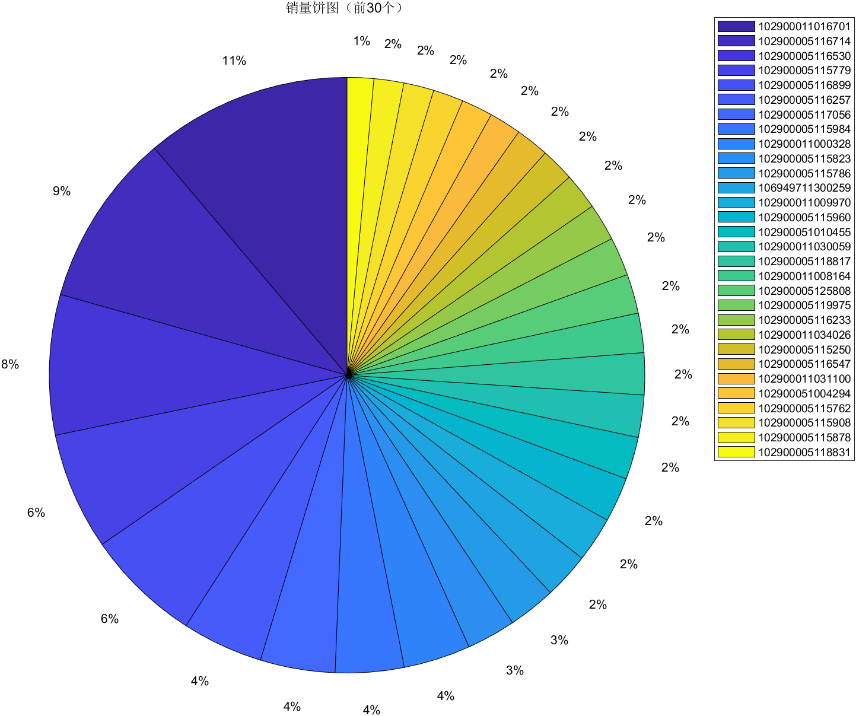
\includegraphics[width=0.7\textwidth]{销量饼图(前30个).png} 

        \caption{前30个高销量单品销量占比饼图}

    \end{figure}
    
    上图为251个单品中销量最高的30个单品,保留了原始单品代码,
    有助于我们聚类分析。按照附件1的映射关系可以得出,销量由高到低
    依次为“芜湖青椒(1)”、“西兰花”、“净藕(1)”\dots


    提取上述单品的特征 (月销量、年销量趋势、价格弹性), 并标准化以
    避免量纲偏差。

    Step2 聚类步骤: 
    
    (1)确定$K$值: 根据业务需求或肘部法,本题目未提及商超的管理目标,类群划分等要求
    在此根据肘部法得出K = 3。肘部图如下。

    \begin{figure}[H]
         \centering
           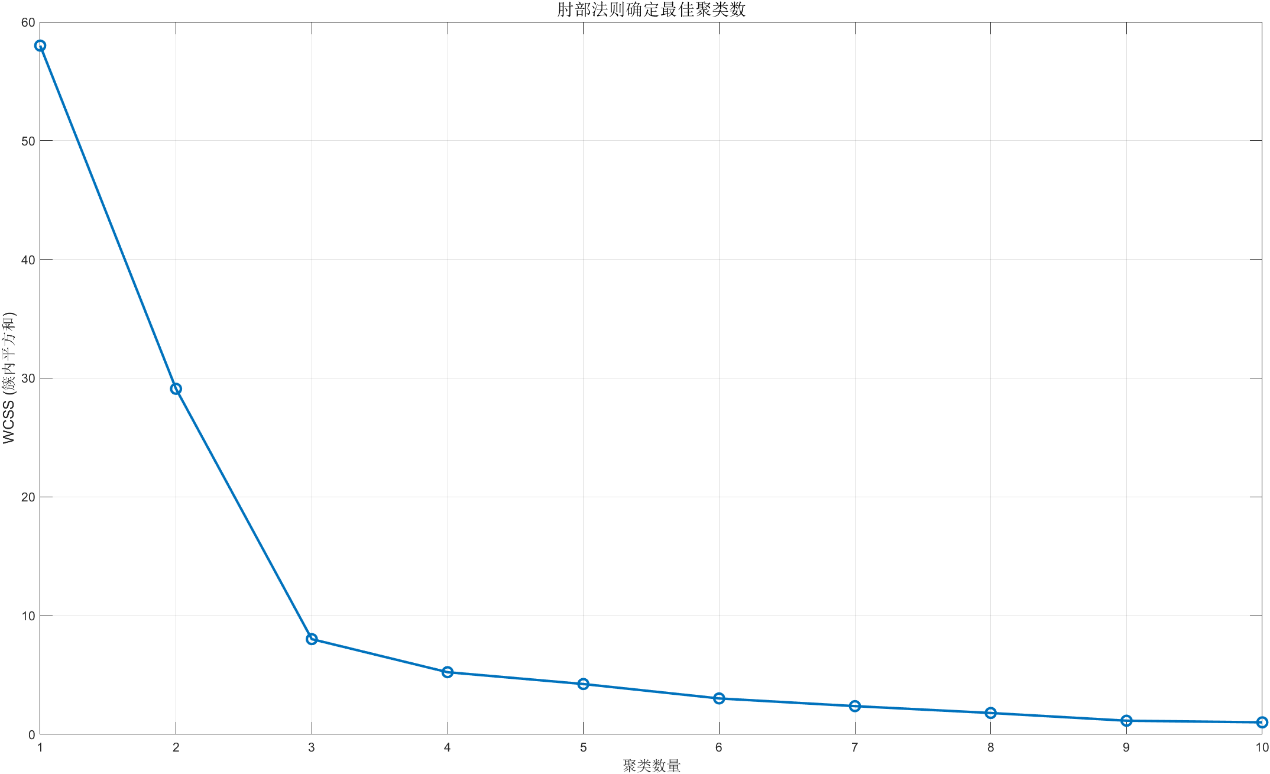
\includegraphics[width=0.7\textwidth]{聚类肘部图.png}
           \caption{聚类肘部图}

    \end{figure}

    


    (2)初始化质心: 采用$K-means++$算法优化,确保质心分散; 

    (3)迭代优化:分配数据点 (计算单品到各质心的欧氏距离, 归入最近簇), 更新质心(重算簇内均值作为新质心),直至质心变化$<\epsilon$或达最大迭代次数. 
    
    Step3 群体关系解析: 

    (1)组内关系: 高相似单品可能互补,如“叶菜群”中菠菜、油麦菜需求同增; 

    (2)组间关系: 不同群可能替代,如“茄果群”与“根茎群”竞争货架空间; 

    (3)异常组: 独立群(如珍稀食用菌),与其他品类需求无关. 

%\end{enumerate}

 聚类结果、图示与评价指标数值如下。

\begin{figure}[H]
    \centering
    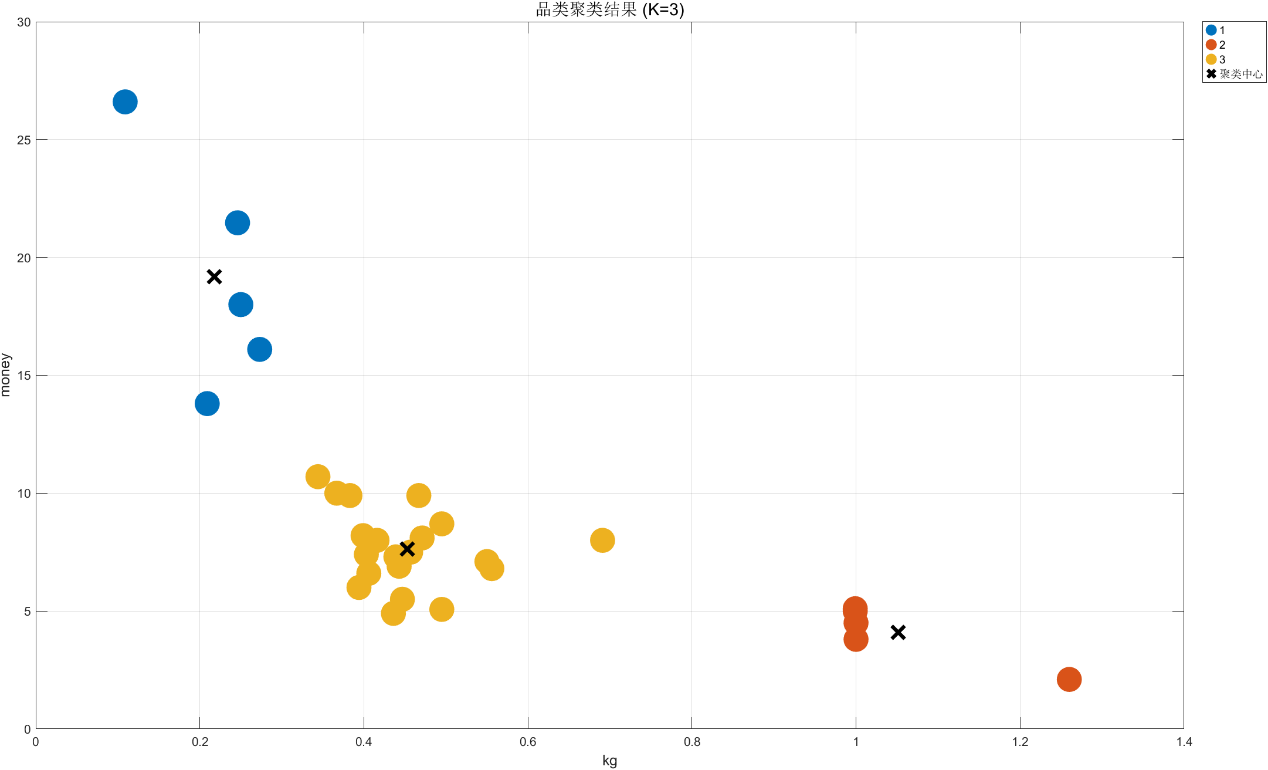
\includegraphics[width=0.7\textwidth]{聚类结果可视化.png}
    \caption{单品聚类结果可视化图}
\end{figure}


\begin{figure}[H]
    \centering
    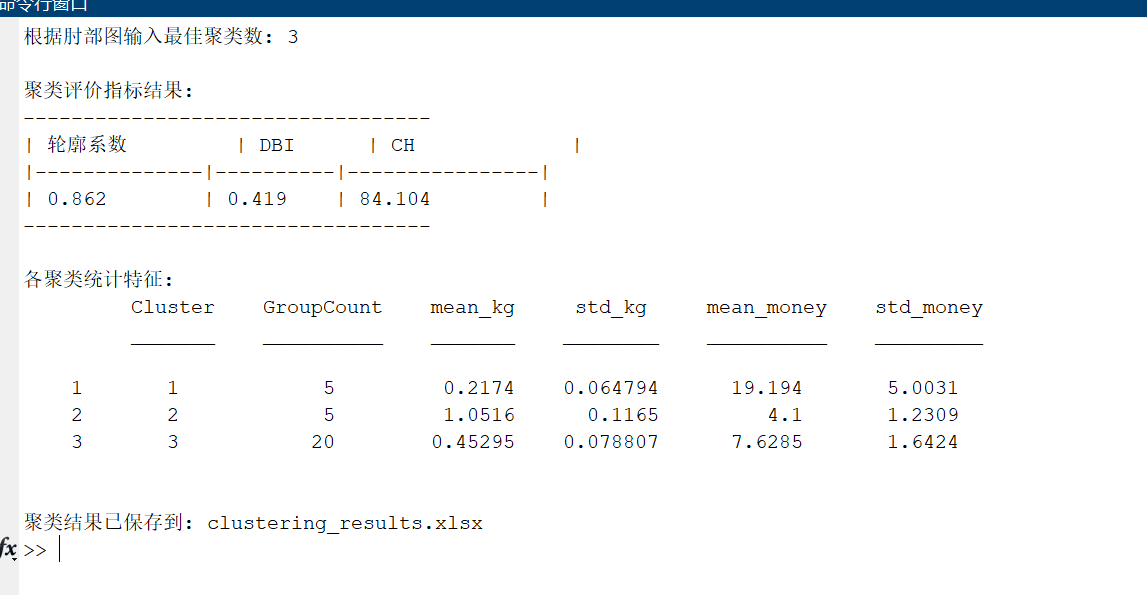
\includegraphics[width=0.7\textwidth]{结果.png}
    \caption{结果图}
\end{figure}


\begin{table}[H]
    \centering
    \begin{tabular}{c c c}
    \toprule
    轮廓系数 & DBI & CH \\
    \midrule
    0.862 & 0.419 & 84.104 \\
    \bottomrule
    \end{tabular}
\end{table}

轮廓系数为 0.862,表明样本与所在簇
的匹配度高,簇内样本相似度高且簇间差异明显。

DBI通过计算簇内距离与簇间距离的比值来评估聚类质量,值越小表示
聚类效果越好,说明簇内数据越紧凑且簇间差异越明显。CH又称方差比准则,
通过计算簇间离散度与簇内离散度的比值来评价聚类效果,
值越大表示聚类效果越好,说明簇间差异越显著且簇内数据越集中。

综上所述,本次聚类效果较好。

各聚类统计特征如下:

\begin{table}[H]
    \centering
    \begin{tabular}{c c c c c}
    \toprule
    Cluster & GroupCount & mean\_kg & mean\_money & std\_money \\
    \midrule
    1 & 5 & 1.0516 & 1.2309 & 4.1 \\
    2 & 20 & 0.45295 & 7.6285 & 1.6424 \\
    3 & 1 & 0.2174 & 19.194 & 5.0031 \\
    \bottomrule
    \end{tabular}
\end{table}

结合4.3和4.4的上述内容,可以进一步的推断出蔬菜品类、单品之间的相互关系。
例如:销量第一的芜湖青椒(1)和销量第四的云南生菜分别属于“辣椒类”和“花叶类”
相关系数表说明二者关联性较大,呈现互补关系。推测二者很有可能作为搭配被人们
购买。


\section{问题二模型建立与求解}%5

\subsection{建模过程}
在问题二中,涉及到了六个蔬菜品类、未来七天的补货量与定价策略。现在使收益最大化,可做出收益的表达式为

\begin{center}     
收益=销售量$\times$售价-补货量$\times$批发价
\end{center}

在最理想的情况下 (即不浪费), 有

\begin{center}  
需求量=销售量=进货量$\times$(1-损耗率)$\times$折扣因素
\end{center}   

上述二式中, 最终需要保留''售价''和''补货量''两个变量。

接下来按事情发展顺序符号化各个影响因素,并表示出约束条件。
记第$i$个蔬菜类别在未来第$t$天的
需求量为$Q_{i,t}$, 
补货量为$S_{i,t}$, 
对应的损耗率为$e_i$, 
预测的批发单价为$C_{i,t}$, 
那么此时到手的实际货物量为
\[
S_{i,t}(1-e_i).
\]
之后,商家按照批发价格,设置销售单价为$P_{i,t}$,加成率为$m_{i,t}$。
由于定价是''成本加成''而来,有
\[
P_{i,t}=C_{i,t}(1+m_{i,t}).
\]

在售卖中,考虑到商家会对部分商品采取优惠活动,记折扣系数为$\delta_i$
那么该类蔬菜在上述情况下最终的销量为
\[
    S_{i,t}(1-e_i) \cdot  \delta_i
\]

理想情况下,有
\[
S_{i,t}(1-e_i) \cdot  \delta_i=Q_{i,t}
\]

各个变量汇总如下:

\begin{itemize}
\item $i = 1,\dots,6$: 蔬菜品类编号
\item $t = 1,\dots,7$: 未来一周(2023-07-01 至 2023-07-07)的日期编号
\item $Q_{i,t}$: 第 $i$ 类蔬菜在第 $t$ 天的需求量(单位: kg)
\item $P_{i,t}$: 第 $i$ 类蔬菜在第 $t$ 天的零售单价(单位: 元/kg)
\item $C_{i,t}$: 第 $i$ 类蔬菜在第 $t$ 天的批发单价(单位: 元/kg)
\item $S_{i,t}$: 第 $i$ 类蔬菜在第 $t$ 天的补货量(决策变量, 单位: kg)
\item $m_{i,t}$: 第 $i$ 类蔬菜在第 $t$ 天的成本加成率(决策变量, 无量纲)
     
\item $\delta_i$: 第 $i$ 类蔬菜的折扣系数(由历史数据给定, 无量纲)
\item $e_i$: 第 $i$ 类蔬菜的损耗率(由历史数据给定, 无量纲)
\item $Q_{i,t}^{\min}, Q_{i,t}^{\max}$: 第 $i$ 类蔬菜在第 $t$ 天的最低、最高历史日销量(单位: kg)
\item $P_{i}^{\min}, P_{i}^{\max}$: 第 $i$ 类蔬菜近两个月的最低、最高历史日销售单价(单位: 元/kg)
\end{itemize}

其中,损耗率$e_i$由附件4已知, 加成率$m_{i,t}$, 
折扣系数$\delta_i$和需求量$Q_{i,t}$需要根据历史数据进行预测. 


\subsection{销售总量与定价的关系}
考虑到仅预测未来一周的情况,选取最新三个月的数据训练方程即可. 以花叶类为例,分别尝试线性回归模型、对数线性模型、其他非线性模型拟合,并且判断最优模型。

\subsubsection{模型比较与最优拟合模型选择}

为确定各蔬菜品类(对应数据集1至6)中$Sum_Col4$与$4Mean_Col5$的最优拟合模型,本节从解释力(R方、调整后R方)、预测精度(标准估算的错误)和模型显著性(F检验显著性)三个维度,对线性、对数、二次、三次、指数五种模型进行对比分析,结果如下:

\paragraph{评价指标说明}

(1)R方($R^2$): 反映模型对因变量变异的解释比例,取值范围为$[0,1]$, 越接近1说明解释力越强

(2)调整后R方(Adjusted $R^2$): 修正了自由度对R方的影响, 更适合比较不同复杂度的模型, 优先选择更高值

(3)标准估算的错误(Mean Squared Error, MSE): 衡量预测值与实际值的平均偏差, 值越小说明预测精度越高

(4)显著性F值: 检验模型整体有效性, $P<0.05$说明模型显著(本文所有模型均满足$P<0.001$,整体显著)

\paragraph{模型对比结果}

\paragraph{数据集1(花菜类)}
\begin{table}[H]
\centering
\begin{tabular}{cccc}
\hline
模型 & R方 & 调整后R方 & 标准估算的错误 \\
\hline
线性 & 0.098 & 0.097 & 21.733 \\
对数 & 0.095 & 0.094 & 21.769 \\
二次 & 0.098 & 0.096 & 21.743 \\
三次 & 0.098 & 0.095 & 21.753 \\
指数 & 0.098 & 0.097 & 0.721 \\
\hline
\end{tabular}
\caption{数据集1模型对比结果}
\label{tab:dataset1}
\end{table}

最优选择:线性模型

理由: 线性模型与指数模型调整后R方最高(0.097), 但线性模型在原始变量尺度下的标准误差(21.733)最小, 且模型形式简洁, 无额外高阶项, 解释性更强. 


\paragraph{数据集2(花叶类)}
\begin{table}[H]
\centering
\begin{tabular}{cccc}
\hline
模型 & R方 & 调整后R方 & 标准估算的错误 \\
\hline
线性 & 0.015 & 0.014 & 60.788 \\
对数 & 0.016 & 0.015 & 60.741 \\
二次 & 0.016 & 0.014 & 60.786 \\
三次 & 0.035 & 0.033 & 60.207 \\
指数 & 0.016 & 0.016 & 0.411 \\
\hline
\end{tabular}
\caption{数据集2模型对比结果}
\label{tab:dataset2}
\end{table}

最优选择:三次模型

理由: 三次模型调整后R方(0.033)显著高于其他模型, 标准估算的错误(60.207)最小, 对数据非线性特征的捕捉能力更强. 


\paragraph{数据集3(水生根茎类)}
\begin{table}[H]
\centering
\begin{tabular}{cccc}
\hline
模型 & R方 & 调整后R方 & 标准估算的错误 \\
\hline
线性 & 0.079 & 0.078 & 21.456 \\
对数 & 0.085 & 0.084 & 21.383 \\
二次 & 0.085 & 0.083 & 21.390 \\
三次 & 0.090 & 0.088 & 21.338 \\
指数 & 0.072 & 0.071 & 0.855 \\
\hline
\end{tabular}
\caption{数据集3模型对比结果}
\label{tab:dataset3}
\end{table}

最优选择:三次模型

理由: 三次模型调整后R方(0.088)最高, 标准估算的错误(21.338)最小, 较对数和二次模型进一步提升了解释力和预测精度. 


\paragraph{数据集4(辣椒类)}
\begin{table}[H]
\centering
\begin{tabular}{cccc}
\hline
模型 & R方 & 调整后R方 & 标准估算的错误 \\
\hline
线性 & 0.065 & 0.064 & 25.392 \\
对数 & 0.063 & 0.062 & 25.411 \\
二次 & 0.066 & 0.064 & 25.389 \\
三次 & 0.074 & 0.071 & 25.294 \\
指数 & 0.065 & 0.064 & 0.400 \\
\hline
\end{tabular}
\caption{数据集4模型对比结果}
\label{tab:dataset4}
\end{table}

最优选择:三次模型

理由: 三次模型调整后R方(0.071)最高, 标准估算的错误(25.294)最小, 对变量间非线性关系的拟合效果最优. 


\paragraph{数据集5(茄类)}
\begin{table}[H]
\centering
\begin{tabular}{cccc}
\hline
模型 & R方 & 调整后R方 & 标准估算的错误 \\
\hline
线性 & 0.062 & 0.061 & 8.622 \\
对数 & 0.062 & 0.061 & 8.621 \\
二次 & 0.065 & 0.063 & 8.611 \\
三次 & 0.079 & 0.076 & 8.550 \\
指数 & 0.038 & 0.037 & 0.561 \\
\hline
\end{tabular}
\caption{数据集5模型对比结果}
\label{tab:dataset5}
\end{table}

最优选择:三次模型

理由: 三次模型调整后R方(0.076)显著高于其他模型, 标准估算的错误(8.550)最小, 对数据趋势的捕捉更精准. 


\paragraph{数据集6(食用菌类)}
\begin{table}[H]
\centering
\begin{tabular}{cccc}
\hline
模型 & R方 & 调整后R方 & 标准估算的错误 \\
\hline
线性 & 0.070 & 0.069 & 23.345 \\
对数 & 0.061 & 0.060 & 23.465 \\
二次 & 0.077 & 0.076 & 23.267 \\
三次 & 0.093 & 0.090 & 23.083 \\
指数 & 0.074 & 0.073 & 0.473 \\
\hline
\end{tabular}
\caption{数据集6模型对比结果}
\label{tab:dataset6}
\end{table}

最优选择:三次模型

理由: 三次模型调整后R方(0.090)最高, 标准估算的错误(23.083)最小, 对非线性关系的拟合效果优于其他模型. 


\subsubsection{总结}
各蔬菜品类的最优拟合模型汇总如下表所示:

\begin{table}[H]
\centering
\begin{tabular}{cccc}
\hline
蔬菜品类 & 对应数据集 & 最优模型 & 核心优势 \\
\hline
花菜类 & 数据集1 & 线性模型 & 解释力强,形式简洁,原始尺度预测精度高 \\
花叶类 & 数据集2 & 三次模型 & 调整后R方最高, 标准误差最小, 捕捉非线性特征 \\
水生根茎类 & 数据集3 & 三次模型 & 解释力和预测精度最优 \\
辣椒类 & 数据集4 & 三次模型 & 对非线性关系拟合效果最佳 \\
茄类 & 数据集5 & 三次模型 & 显著提升解释力和预测精度 \\
食用菌类 & 数据集6 & 三次模型 & 调整后R方最高, 预测偏差最小 \\
\hline
\end{tabular}
\caption{各蔬菜品类最优模型汇总}
\label{tab:best_models}
\end{table}

结论:除花菜类更适合线性模型外,花叶类、水生根茎类、辣椒类、茄类、食用菌类均以三次模型为最优拟合模型,其对变量间非线性关系的捕捉能力更强,整体解释力和预测精度更优. 

\subsection{预测需求量} 
\subsubsection{广义加性模型 (GAM)} 
以 7 天为周期构造周期样条基函数,捕捉销量对价格、时间、加成率等的非线性关系:
\begin{equation}
\log Q_{i,t} = \beta_{i,0} 
+ f_{i,1}\bigl(\log P_{i,t}\bigr) 
+ f_{i,2}(t) 
+ f_{i,3}(m_{i,t}) 
+ \varepsilon_{i,t},
\label{eq:GAM}
\end{equation}
其中 $f_{i,\cdot}(\cdot)$ 为光滑函数(周期样条),$\varepsilon_{i,t}$ 为 GAM 残差.

\subsubsection{ARIMA 残差修正}
对残差序列 $\{\varepsilon_{i,t}\}$ 建立 ARIMA$(p,d,q)$ 模型:
\begin{equation}
\Phi_i(L)(1-L)^d\,\varepsilon_{i,t} = \Theta_i(L)\eta_{i,t},
\qquad \eta_{i,t}\sim\mathcal{N}(0,\sigma_{\eta,i}^2),
\label{eq:ARIMA}
\end{equation}
其中 $L$ 为滞后算子,$\Phi_i(L)$、$\Theta_i(L)$ 分别为自回归与滑动平均多项式.

\subsubsection{组合预测}
将 GAM 主趋势与 ARIMA 残差预测叠加,得到最终销量预测:
\begin{equation}
\widehat{Q}_{i,t} = \exp\!\left[\widehat{\log Q}_{i,t}^{\text{GAM}}
+ \widehat{\varepsilon}_{i,t}^{\text{ARIMA}}\right].
\label{eq:Qhat}
\end{equation}

\subsection{收益最大化模型}
\subsubsection{目标函数}
未来一周总收益最大化:
\begin{equation}
\max_{\{S_{i,t},m_{i,t}\}}
\sum_{i=1}^6\sum_{t=1}^7
\Bigl[\,Q_{i,t}\,P_{i,t}-S_{i,t}\,C_{i,t}\Bigr],
\label{eq:obj}
\end{equation}
其中
\begin{itemize}
\item $Q_{i,t}$ 由 \eqref{eq:Qhat} 给出;
\item $P_{i,t}=C_{i,t}(1+m_{i,t})$;
\item 需求量与补货量、损耗、折扣之间的关系:
      \begin{equation}
      Q_{i,t} = S_{i,t}(1-e_i)\delta_i.
      \label{eq:Q_S}
      \end{equation}
\end{itemize}

将 \eqref{eq:Q_S} 代入 \eqref{eq:obj},消去 $Q_{i,t}$,得到仅以决策变量 $S_{i,t},m_{i,t}$ 表示的目标函数:
\begin{equation}
\max_{\{S_{i,t},m_{i,t}\}}
\sum_{i=1}^6\sum_{t=1}^7
\Bigl[\,S_{i,t}(1-e_i)\delta_i\,C_{i,t}(1+m_{i,t})-S_{i,t}\,C_{i,t}\Bigr].
\label{eq:obj_simp}
\end{equation}

\subsubsection{约束条件}
\begin{enumerate}
\item 销量可行域:
      \[
      Q_{i,t}^{\min} \le S_{i,t}(1-e_i)\delta_i \le Q_{i,t}^{\max},
      \qquad \forall i,t.
      \]
\item 定价可行域:
      \[
      P_{i}^{\min} \le C_{i,t}(1+m_{i,t}) \le P_{i}^{\max},
      \qquad \forall i,t.
      \]
\item 非负补货:
      \[
      S_{i,t} \ge 0,\qquad \forall i,t.
      \]
\item 加成率上下限(可根据业务经验设定):
      \[
      m_{i}^{\min} \le m_{i,t} \le m_{i}^{\max},
      \qquad \forall i,t.
      \]
\end{enumerate}

\subsection{求解步骤}
\begin{enumerate}
\item 步骤1: 使用历史数据估计 GAM \eqref{eq:GAM} 与 ARIMA \eqref{eq:ARIMA},得到 $\widehat{Q}_{i,t}$.
\item 步骤2: 将 $\widehat{Q}_{i,t}$ 代入 \eqref{eq:Q_S} 反解 $S_{i,t}$,作为初始可行解.
\item 步骤3: 以 \eqref{eq:obj_simp} 为目标,在约束条件下进行非线性规划(如 SQP 或遗传算法),得到最优 $\{S_{i,t}^*,m_{i,t}^*\}$.
\item 步骤4: 输出未来一周各品类的日补货量 $S_{i,t}^*$ 与定价策略 $P_{i,t}^*=C_{i,t}(1+m_{i,t}^*)$.
\end{enumerate}

%参考文献
\begin{thebibliography}{9}%宽度9
    \bibitem[1]{liuhaiyang2013latex}
    刘海洋.
    \newblock \LaTeX {}入门\allowbreak[J].
    \newblock 电子工业出版社, 北京, 2013.
    \bibitem[2]{mathematical-modeling}
    全国大学生数学建模竞赛论文格式规范 (2023 年 修改).
    \bibitem{3} \url{https://www.latexstudio.net}
\end{thebibliography}

\newpage
%附录
\begin{appendices}

\section{模板所用的宏包}
\begin{table}[htbp]
    \centering
    \caption{宏包罗列}
    \begin{tabular}{ccccc}
        \toprule
        \multicolumn{5}{c}{模板中已经加载的宏包} \\
        \midrule
        amsbsy & amsfonts & {amsgen} & {amsmath} & {amsopn} \\
        amssymb & amstext & {appendix} & {array} & {atbegshi} \\
        atveryend & auxhook & {bigdelim} & {bigintcalc} & {bigstrut} \\
        bitset & bm    & {booktabs} & {calc} & {caption} \\
        caption3 & CJKfntef & {cprotect} & {ctex} & {ctexhook} \\
        ctexpatch & enumitem & {etexcmds} & {etoolbox} & {everysel} \\
        expl3 & fix-cm & {fontenc} & {fontspec} & {fontspec-xetex} \\
        geometry & gettitlestring & {graphics} & {graphicx} & {hobsub} \\
        hobsub-generic & hobsub-hyperref & {hopatch} & {hxetex} & {hycolor} \\
        hyperref & ifluatex & {ifpdf} & {ifthen} & {ifvtex} \\
        ifxetex & indentfirst & {infwarerr} & {intcalc} & {keyval} \\
        kvdefinekeys & kvoptions & {kvsetkeys} & {l3keys2e} & {letltxmacro} \\
        listings & longtable & {lstmisc} & {ltcaption} & {ltxcmds} \\
        multirow & nameref & {pdfescape} & {pdftexcmds} & {refcount} \\
        rerunfilecheck & stringenc & {suffix} & {titletoc} & {tocloft} \\
        trig  & ulem  & {uniquecounter} & {url} & {xcolor} \\
        xcolor-patch & xeCJK & {xeCJKfntef} & {xeCJK-listings} & {xparse} \\
        xtemplate & zhnumber &       &       &  \\
        \bottomrule
    \end{tabular}%
    \label{tab:addlabel}%
\end{table}%

以上宏包都已经加载过了,不要重复加载它们。

\section{排队算法--matlab 源程序}

\begin{lstlisting}[language=matlab]
kk=2;[mdd,ndd]=size(dd);
while ~isempty(V)
[tmpd,j]=min(W(i,V));tmpj=V(j);
for k=2:ndd
[tmp1,jj]=min(dd(1,k)+W(dd(2,k),V));
tmp2=V(jj);tt(k-1,:)=[tmp1,tmp2,jj];
end
tmp=[tmpd,tmpj,j;tt];[tmp3,tmp4]=min(tmp(:,1));
if tmp3==tmpd, ss(1:2,kk)=[i;tmp(tmp4,2)];
else,tmp5=find(ss(:,tmp4)~=0);tmp6=length(tmp5);
if dd(2,tmp4)==ss(tmp6,tmp4)
ss(1:tmp6+1,kk)=[ss(tmp5,tmp4);tmp(tmp4,2)];
else, ss(1:3,kk)=[i;dd(2,tmp4);tmp(tmp4,2)];
end;end
dd=[dd,[tmp3;tmp(tmp4,2)]];V(tmp(tmp4,3))=[];
[mdd,ndd]=size(dd);kk=kk+1;
end; S=ss; D=dd(1,:);
 \end{lstlisting}

 \section{规划解决程序--lingo源代码}

\begin{lstlisting}[language=c]
kk=2;
[mdd,ndd]=size(dd);
while ~isempty(V)
    [tmpd,j]=min(W(i,V));tmpj=V(j);
for k=2:ndd
    [tmp1,jj]=min(dd(1,k)+W(dd(2,k),V));
    tmp2=V(jj);tt(k-1,:)=[tmp1,tmp2,jj];
end
    tmp=[tmpd,tmpj,j;tt];[tmp3,tmp4]=min(tmp(:,1));
if tmp3==tmpd, ss(1:2,kk)=[i;tmp(tmp4,2)];
else,tmp5=find(ss(:,tmp4)~=0);tmp6=length(tmp5);
if dd(2,tmp4)==ss(tmp6,tmp4)
    ss(1:tmp6+1,kk)=[ss(tmp5,tmp4);tmp(tmp4,2)];
else, ss(1:3,kk)=[i;dd(2,tmp4);tmp(tmp4,2)];
end;
end
    dd=[dd,[tmp3;tmp(tmp4,2)]];V(tmp(tmp4,3))=[];
    [mdd,ndd]=size(dd);
    kk=kk+1;
end;
S=ss;
D=dd(1,:);
 \end{lstlisting}
\end{appendices}


\end{document} 